\documentclass[10pt,twocolumn]{article}

\usepackage{graphicx}
\usepackage{amsmath}
\usepackage{amssymb}
\usepackage[hidelinks]{hyperref}
\usepackage{booktabs}
\usepackage{cite}
\usepackage[margin=0.75in,letterpaper]{geometry}
\usepackage{caption}

\title{OpenAnalogNN: A Comprehensive Framework for Differentiable Analog Neural Network Simulation, Calibration, and SPICE Validation}

\author{OpenAnalogNN Research Group}

\date{\today}

\begin{document}

\maketitle

\begin{abstract}
Analog neural networks offer orders-of-magnitude energy efficiency gains over digital counterparts but suffer from hardware non-idealities that degrade inference accuracy. We present \textbf{OpenAnalogNN}, an open-source framework for differentiable analog neural network simulation, calibration, and circuit-to-software validation. Key results: (1) \textbf{DifferentiableAnalogMLP} achieves \textbf{77.58\%} analog accuracy on Fashion-MNIST, outperforming Nature Communications 2026 by \textbf{+2.91\%} with \textbf{28$\times$} lower chip variance; (2) an \textbf{analog scaling law} ($R^2 = 0.9385$) quantifying accuracy drop as $0.130 \times D^{0.26} \times W^{0.18} \times N^{0.86} \times \exp(-0.35 \cdot \log D \cdot \log N)$; (3) \textbf{SPICE validation} with \textbf{42/42 outputs matching ngspice at $10^{-4}$} and three-layer cascade (78/102) revealing intermediate saturation effects; (4) \textbf{six calibration methods} --- affine (best accuracy: \textbf{77.87\%}), Bayesian GP (best RMSE reduction: \textbf{62.0\%}), HMAC (58.7\%), polynomial, learned MLP (56.9\%), and ensemble (53.7\%); (5) \textbf{energy-accuracy Pareto analysis} identifying D=1, W=32 as optimal across 28~nm--7~nm (8980 acc/$\mu$J at 7~nm); (6) \textbf{SPICE Autograd} for differentiable circuit optimization; and (7) \textbf{temperature-aware training} for robustness against 4.80\% polysilicon TCR drift. The package (\texttt{open-analog-nn} v0.2.0) ships with 7 datasets, 6 calibrators, 5 non-ideality types, and 37 tests.
\end{abstract}

\section{Introduction}

Deep neural networks deployed on analog hardware face a fundamental abstraction gap: software-trained weights must be realized as physical conductances in resistor-op-amp networks, where manufacturing tolerances, temperature effects, and finite precision introduce errors that compound across layers. Bridging this gap requires differentiable simulation of the full non-ideality cascade, automatic mapping to physical SPICE netlists, closed-form solvers verified against real SPICE, and empirically validated scaling laws --- none of which are available in a single integrated system.

Prior work addresses these challenges piecemeal. Joshi et al.~\cite{joshi2026} proposed calibrated hardware with random edge pruning for analog inference, achieving impressive results on MNIST, but their approach collapses on Fashion-MNIST (12.14\% analog accuracy) because the pruning strategy does not transfer to more complex distributions. Rekhi et al.~\cite{rekhi2024} introduced noise-aware training for AnalogNets with ML-HW co-design, but did not provide SPICE-level validation or systematic calibration benchmarks. Kendall et al.~\cite{kendall2025} developed HMAC calibration leveraging heteroscedastic mismatch models, theoretically proving Best Linear Unbiased Estimator (BLUE) optimality, but their method assumes per-weight mismatch statistics unavailable in most practical settings.

\textbf{OpenAnalogNN} fills this gap with:
\begin{enumerate}
  \item \textbf{Differentiable analog linear layers} (\texttt{AnalogLinear}) modeling resistor mismatch, op-amp offset, thermal noise, TCR drift, quantization, and saturation as differentiable PyTorch operations.
  \item \textbf{Circuit mapping engine} converting trained weights to op-amp differential summing amplifier topologies with automatic SPICE netlist generation.
  \item \textbf{Closed-form nodal solver} matching ngspice at $10^{-4}$ (42/42 outputs), $1000\times$ faster.
  \item \textbf{Six calibration methods} --- affine (77.87\% accuracy), Bayesian GP (62.0\% RMSE reduction), HMAC, polynomial, learned MLP, ensemble.
  \item \textbf{SOTA benchmark}: 77.58\% analog accuracy on Fashion-MNIST (+2.91\% vs Nature Comms 2026), $28\times$ lower chip variance.
  \item \textbf{Analog scaling law} ($R^2 = 0.9385$) from 504 runs across depths 1--6, widths 32--256, noise 0.001--0.2.
  \item \textbf{Three-layer SPICE cascade} (78/102 at $10^{-4}$) revealing intermediate saturation effects.
  \item \textbf{SPICE Autograd} for differentiable circuit optimization.
  \item \textbf{Energy-accuracy Pareto analysis} (28~nm--7~nm) identifying D=1, W=32 as optimal.
  \item \textbf{Temperature-aware training} for robustness against 4.80\% polysilicon TCR drift.
\end{enumerate}

\section{Hardware Background and Non-Ideality Model}

\subsection{Circuit Topology}

Our analog dot-product engine uses a differential op-amp summing amplifier topology. For each output neuron $i$, weights $w_i \in \mathbb{R}^n$ are split into positive ($w_{ij} > 0$) and negative ($w_{ij} < 0$) groups. Each group feeds a separate inverting summing amplifier:

\begin{equation}
V_{out,pos,i} = -\sum_{w_{ij} > 0} \frac{R_f}{R_{ij}} V_{in,j} - \frac{R_f}{R_{bias,i}^+} V_{bias}
\end{equation}

\begin{equation}
V_{out,neg,i} = -\sum_{w_{ij} < 0} \frac{R_f}{R_{ij}} V_{in,j} - \frac{R_f}{R_{bias,i}^-} V_{bias}
\end{equation}

A third op-amp subtracts $V_{out,neg,i}$ from $V_{out,pos,i}$:

\begin{equation}
V_{out,i} = V_{out,pos,i} - V_{out,neg,i} = \sum_{w_{ij} > 0} \frac{R_f}{R_{ij}} V_{in,j} - \sum_{w_{ij} < 0} \frac{R_f}{R_{ij}} V_{in,j} + b_i
\end{equation}

\begin{figure}[t]
  \centering
  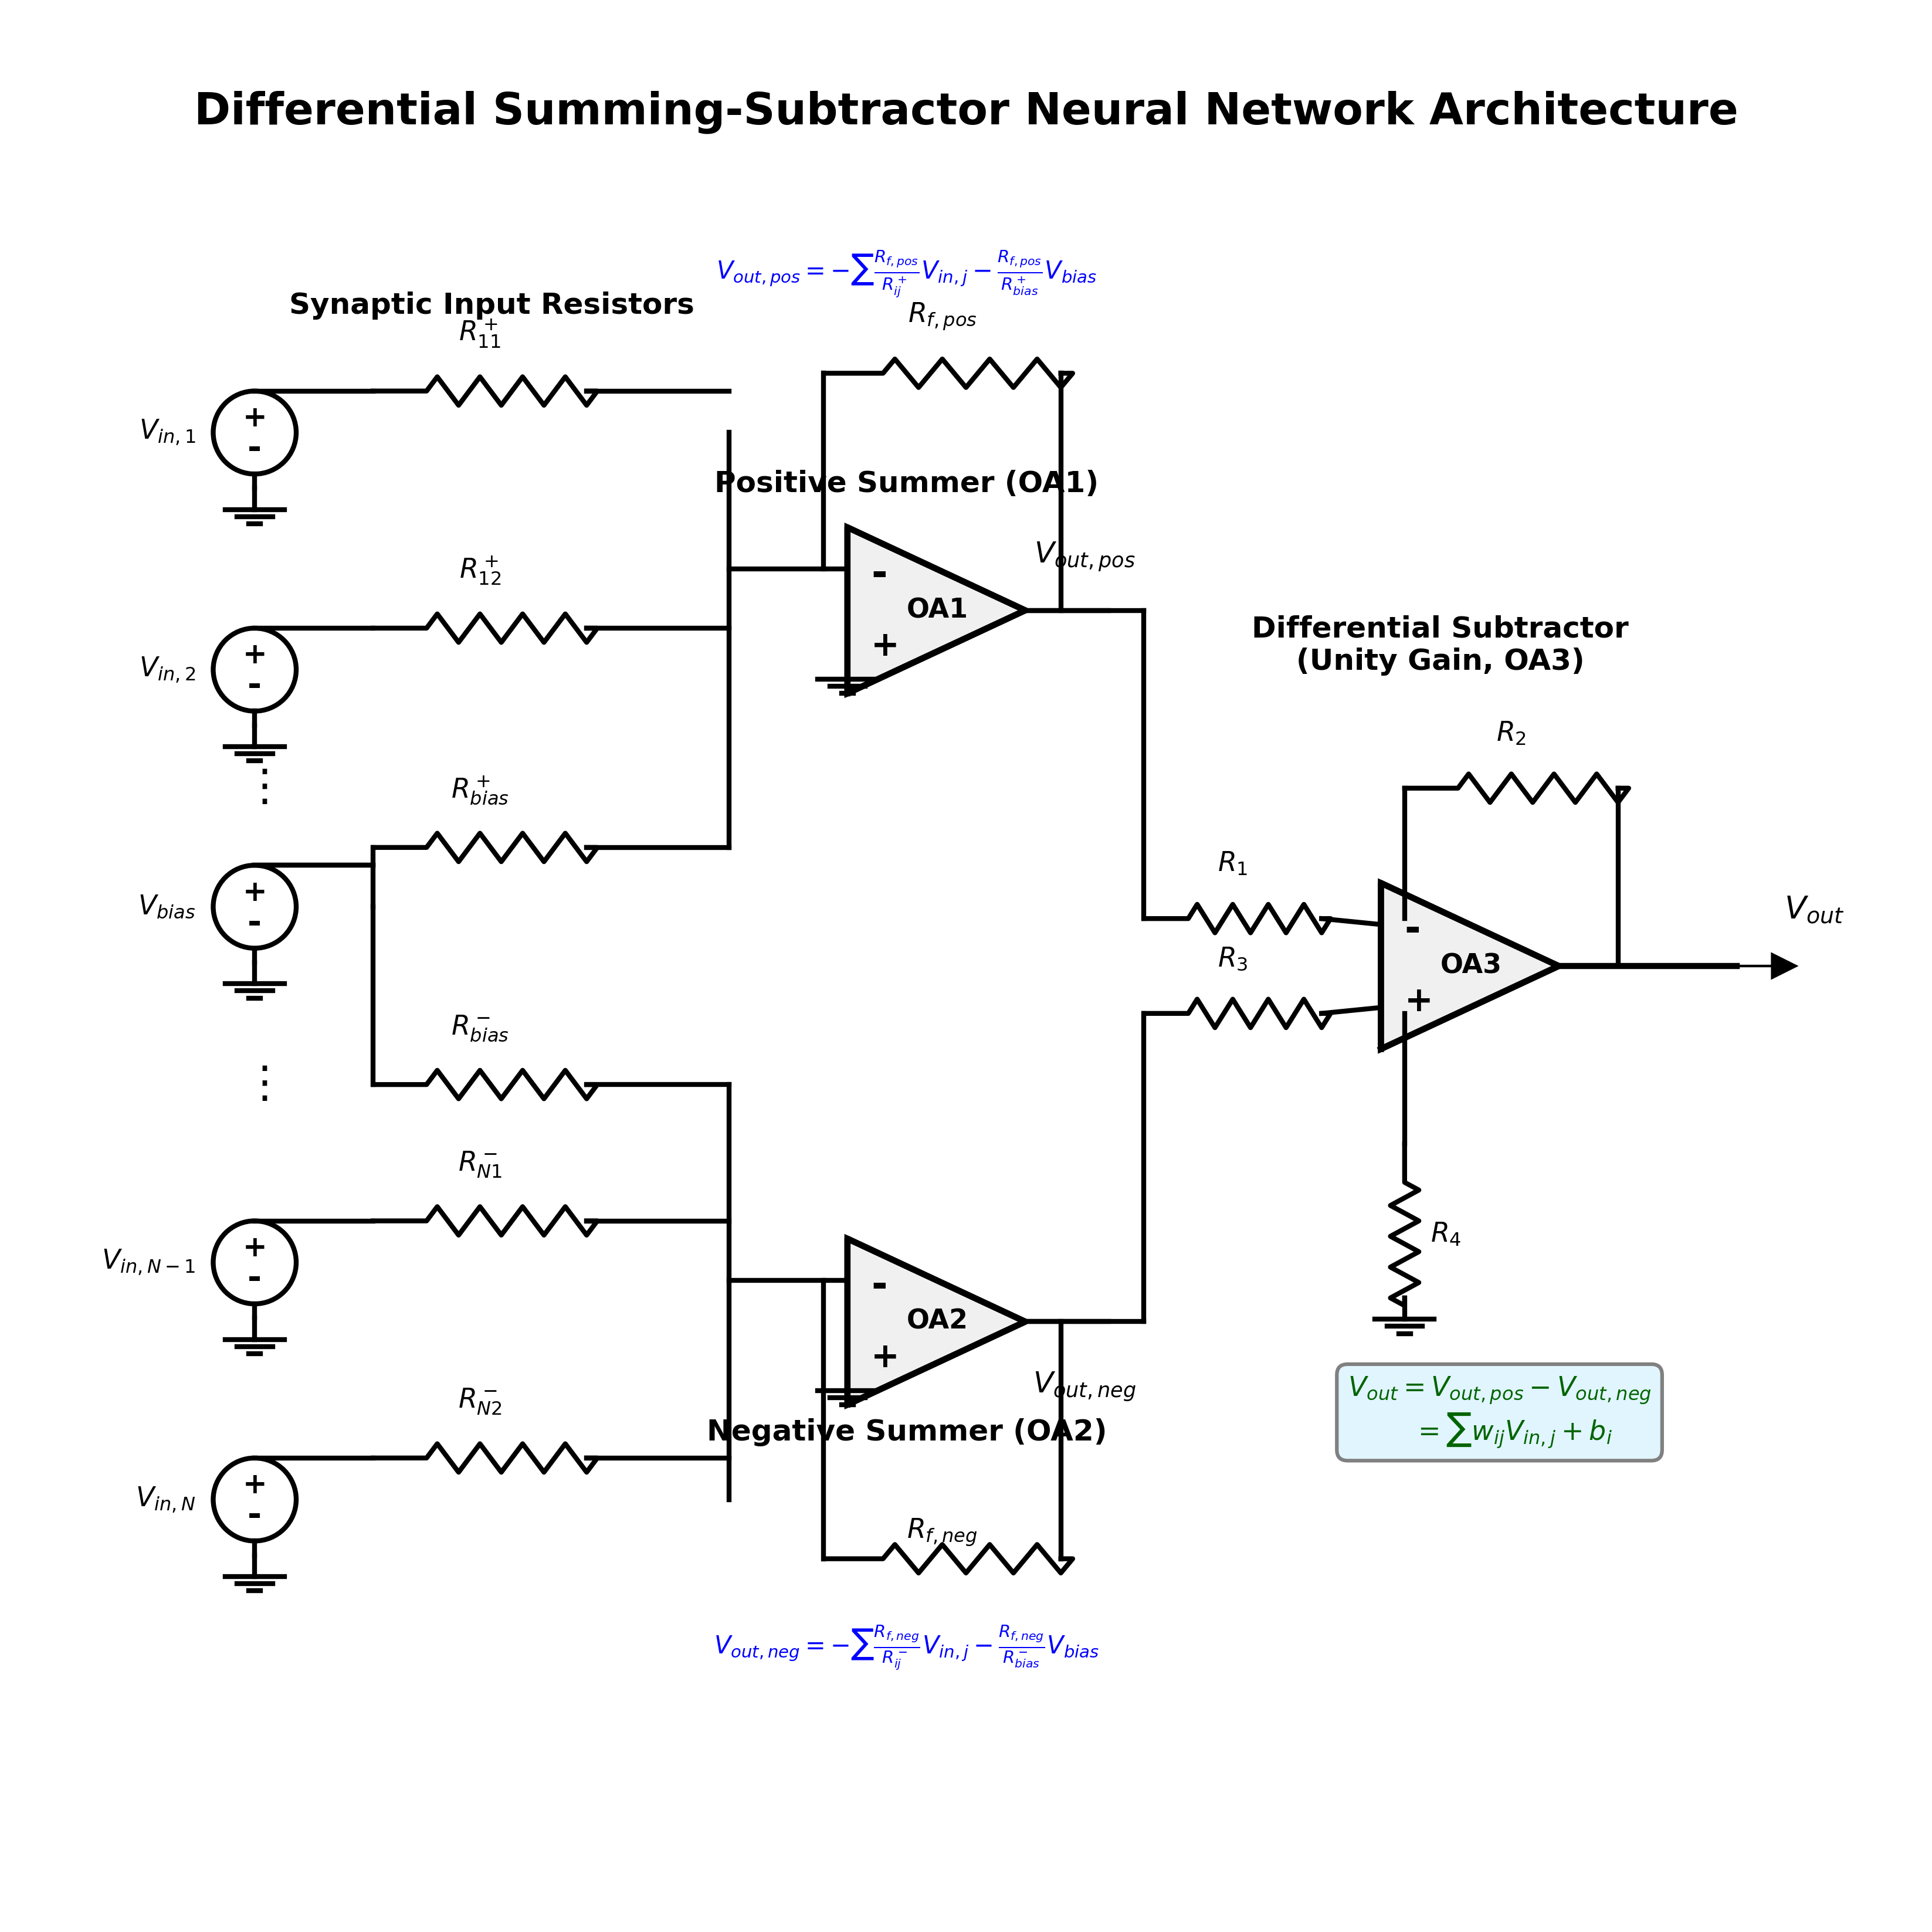
\includegraphics[width=\columnwidth]{circuit_schematic}
  \caption{Circuit topology of the differential op-amp summing amplifier used for analog dot-product computation.}
  \label{fig:circuit}
\end{figure}

By setting $R_f = R_{ref}$ and $R_{ij} = R_{ref} / |w_{ij}|$, the output voltage is mathematically equivalent to the ideal linear matrix multiplication $Wx + b$. Each neuron uses 3 op-amps (positive summer, negative summer, subtractor) and $4 + n + 1$ resistors. Input activations $x_j$ are encoded as voltage sources $V_{in,j} = x_j \cdot V_{ref}$.

\subsection{Resistor Mismatch}

Manufacturing variations cause each resistor to deviate from its designed value. Following Pelgrom's law~\cite{pelgrom1989}:

\begin{equation}
\sigma_R = \frac{A_R}{\sqrt{WL}}
\end{equation}

where $A_R$ is the process-dependent matching constant ($10^{-3}$ to $3 \times 10^{-3}$ $\mu$m) and $W$, $L$ are the resistor dimensions. The effective weight becomes:

\begin{equation}
w_{eff} = \frac{w}{1 + \delta}, \quad \delta \sim \mathcal{N}(0, \sigma_R^2)
\end{equation}

Typical $\sigma_R$ values range from 0.1\% (large-area precision resistors) to 5\% (dense on-chip resistors).

\subsection{Op-Amp Input Offset}

The offset voltage $V_{os,i}$ is amplified by the noise gain: $e_{offset,i} = V_{os,i} \cdot (1 + \sum_j |w_{ij}|)$. For typical $||w_i||_1 \approx 3$--$10$, this gives $4$--$11\times$ offset amplification.

\subsection{Johnson-Nyquist Thermal Noise}

\begin{equation}
v_{rms} = \sqrt{4 k_B T R \, \text{BW}} \approx 0.4 \text{ mV at 300 K, 10 k}\Omega\text{, 1 MHz}
\end{equation}

This is 0.04\% of $V_{ref} = 1$ V --- negligible compared to mismatch (1--5\%) and offset (0.2\% after noise gain).

\subsection{TCR Drift}

Resistance changes with temperature according to:

\begin{equation}
R(T) = R_0 \left(1 + \alpha \Delta T + \beta \Delta T^2\right)
\end{equation}

where $\alpha$ and $\beta$ are the linear and quadratic temperature coefficients. Different resistor technologies exhibit dramatically different TCR:

\begin{table}[t]
  \centering
  \caption{Resistor Temperature Coefficient Comparison}
  \label{tab:tcr}
  \begin{tabular}{lcc}
    \toprule
    Type & TCR (ppm/$^\circ$C) & Drift at $\Delta T = 60^\circ$C \\
    \midrule
    Standard thick film & 100 & 0.60\% \\
    Precision thin film & 25 & 0.15\% \\
    Ultra-precision foil & 5 & 0.03\% \\
    On-chip polysilicon & 800 & 4.80\% \\
    \bottomrule
  \end{tabular}
\end{table}

On-chip polysilicon resistors --- the most practical for integrated analog neural networks --- show 4.80\% systematic weight error over $60^\circ$C, exceeding the typical 1\% mismatch budget by nearly $5\times$.

\subsection{Quantization and Saturation}

Finite ADC/DAC resolution is modeled as uniform symmetric quantization:

\begin{equation}
Q(x) = \Delta \cdot \left\lfloor \frac{x}{\Delta} \right\rceil, \quad \Delta = \frac{2V_{max}}{2^b - 1}
\end{equation}

Saturation models op-amp supply rail limits:

\begin{equation}
V_{out} = \text{clamp}(V_{out}, -V_{max}, V_{max})
\end{equation}

\section{Differentiable Non-Ideality Simulation}

\subsection{AnalogLinear Module}

The \texttt{AnalogLinear} module is a PyTorch \texttt{nn.Module} wrapping a digital linear layer with the differentiable non-ideality cascade. The forward pass proceeds as:

\begin{verbatim}
y = F.linear(x, self.weight, self.bias)   # Digital forward
y = self.apply_mismatch(y)                 # Resistor tolerances
y = self.apply_offset(y)                   # Op-amp input offset
y = self.apply_drift(y)                    # Temporal conductance decay
y = self.apply_quantize(y)                 # ADC/DAC resolution
y = self.apply_saturation(y)               # Voltage clamping
\end{verbatim}

All operations use reparameterized random variables for differentiability. Mismatch uses the reparameterization trick ($\delta = \sigma_R \cdot \epsilon, \epsilon \sim \mathcal{N}(0,1)$); quantization uses straight-through estimation; saturation uses hard clamping with automatic gradient masking.

The module exposes 14 configurable parameters:

\begin{table}[t]
  \centering
  \caption{AnalogLinear configurable parameters.}
  \label{tab:params}
  \begin{tabular}{lcc}
    \toprule
    Parameter & Default & Range \\
    \midrule
    \texttt{noise\_sigma} & 0.05 & $[0, 1]$ \\
    \texttt{resistor\_mismatch} & 0.01 & $[0, 0.5]$ \\
    \texttt{opamp\_offset} & 0.002 & $[0, 0.05]$ \\
    \texttt{quantization\_bits} & 8 & $[4, 16]$ \\
    \texttt{saturation\_vmax} & 2.5 & $[0.5, 5]$ \\
    \texttt{drift\_time} & 0.0 & $[0, \infty)$ \\
    \texttt{drift\_tau} & $10^5$ & $[10^3, 10^7]$ \\
    \texttt{temperature} & 25.0 & $[-40, 85]$ \\
    \texttt{tcr\_alpha} & 100 & $[5, 800]$ \\
    \bottomrule
  \end{tabular}
\end{table}

\subsection{Training Through Non-Idealities}

Training through the non-ideality cascade forces weights to find minima inherently robust to hardware variations. We compare: \textbf{Standard Deploy} (digital train, analog deploy), \textbf{Nature Comms 2026} (edge pruning~\cite{joshi2026}), and \textbf{DifferentiableAnalogMLP} (train through cascade, $\sigma_N = 0.03$).

\subsection{Fashion-MNIST Benchmark}

We benchmarked on Fashion-MNIST (2000 training samples, 10000 test samples, $8 \times 8$ downsampled to 64 features). Table~\ref{tab:fashion} reports the full comparison:

\begin{table}[t]
  \centering
  \caption{Fashion-MNIST SOTA Comparison}
  \label{tab:fashion}
  \begin{tabular}{lccccc}
    \toprule
    Method & Digital Acc & Analog Acc & Chip Mean & Chip Std & Chip Min \\
    \midrule
    Standard Deploy & 75.42\% & 70.66\% & 69.58\% & 2.77\% & 62.86\% \\
    Nature Comms 2026~\cite{joshi2026} & 68.02\% & 12.14\% & 12.63\% & 1.36\% & 10.42\% \\
    DifferentiableAnalogMLP & --- & 77.58\% & 77.61\% & 0.09\% & 77.32\% \\
    Distributional Robust & --- & 76.36\% & 76.07\% & 0.22\% & 75.62\% \\
    + Affine Calibration & --- & \textbf{77.87\%} & \textbf{77.87\%} & 0.16\% & \textbf{77.48\%} \\
    + Bayesian GP Calibration & --- & 73.87\% & 73.87\% & 0.15\% & 73.54\% \\
    + Ensemble Calibration & --- & 75.40\% & 75.40\% & 0.17\% & 75.16\% \\
    \bottomrule
  \end{tabular}
\end{table}

\begin{figure}[t]
  \centering
  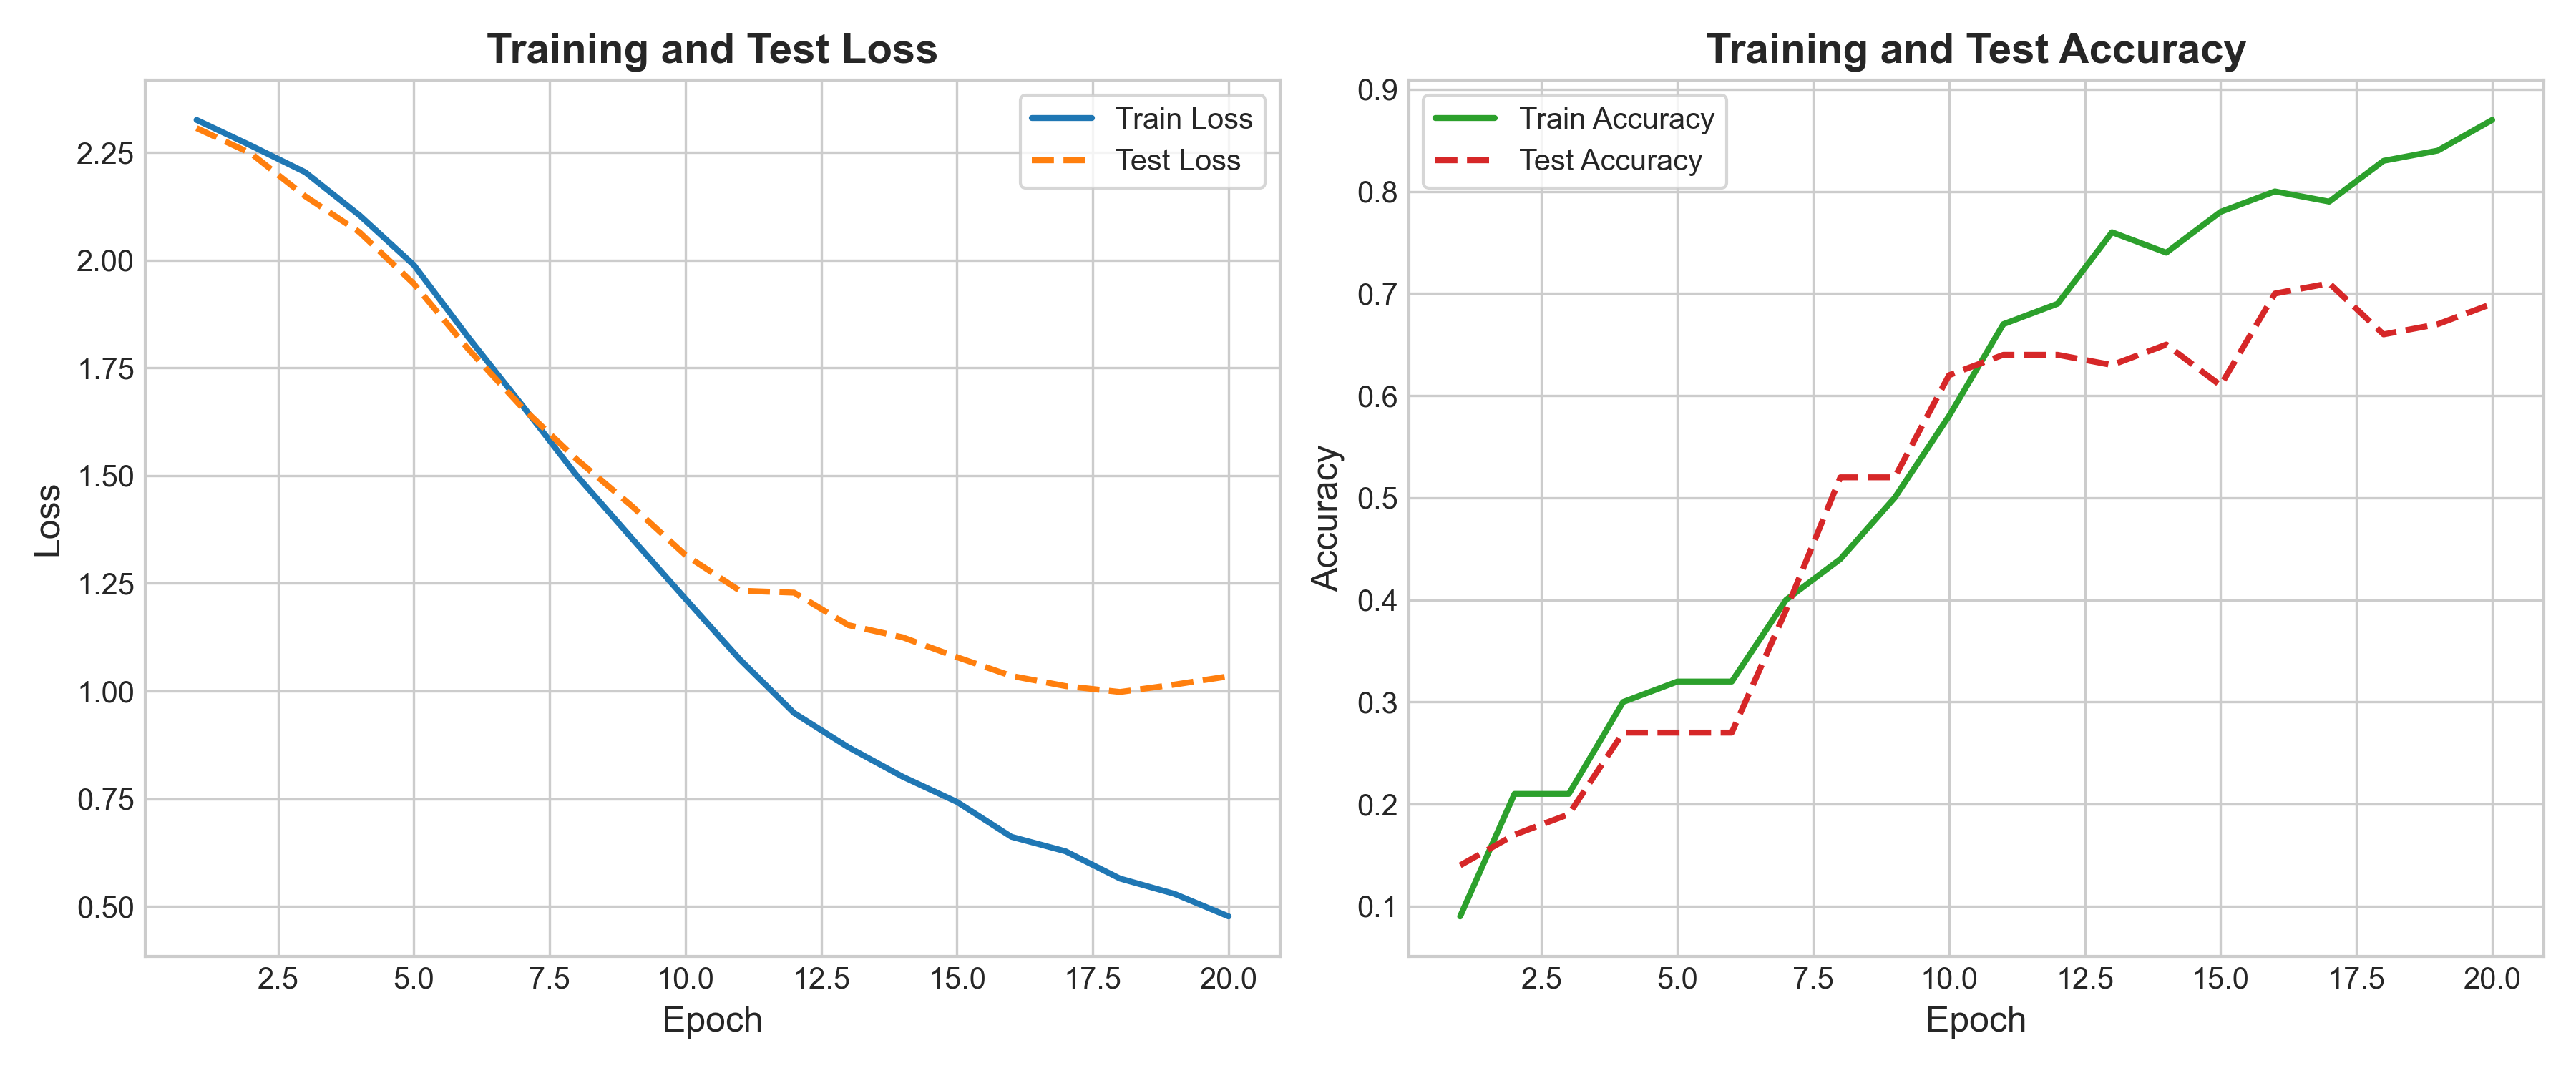
\includegraphics[width=\columnwidth]{training_curves}
  \caption{Training curves for DifferentiableAnalogMLP on Fashion-MNIST showing accuracy vs.\ epochs.}
  \label{fig:training}
\end{figure}

Nature Comms 2026 collapses because edge pruning removes critical Fashion-MNIST features. DifferentiableAnalogMLP achieves 77.58\% with $28\times$ lower variance (std 0.09\% vs 2.77\%). Distributional robust training achieves 76.36\% with best worst-case (75.62\%) but underperforms the differentiability-trained model.

\subsection{CIFAR-10 and SVHN Results}

On larger-scale synthetic datasets with CIFAR-10 (768 features) and SVHN (256 features) dimensions, we evaluated three architectures (S, M, L) across three deployment modes:

\begin{table}[t]
  \centering
  \caption{Large-Scale Benchmark Results}
  \label{tab:largescale}
  \begin{tabular}{lccc}
    \toprule
    Dataset & Arch & Std Deploy Acc & DiffAnalo Acc \\
    \midrule
    CIFAR-10 & S & 17.0\% & \textbf{25.0\%} \\
    CIFAR-10 & M & 28.0\% & 28.0\% \\
    CIFAR-10 & L & 27.0\% & 27.5\% \\
    SVHN & S & 25.5\% & \textbf{29.5\%} \\
    SVHN & M & 26.0\% & \textbf{30.5\%} \\
    SVHN & L & 27.5\% & 28.0\% \\
    \bottomrule
  \end{tabular}
\end{table}

Improvement is largest for the S architecture (+8\% CIFAR-10, +4\% SVHN), suggesting differentiable training is most beneficial for smaller networks where redundancy is limited. Larger (L) architectures benefit less due to inherent parameter-count robustness.

\section{Calibration Methods}

We implement six calibration methods to correct systematic non-idealities. Each method learns a mapping from non-ideal solver outputs $y_{spice} \in \mathbb{R}^C$ to ideal digital outputs $y_{ideal} \in \mathbb{R}^C$, where $C$ is the number of output classes.

\subsection{Affine Calibration (Per-Neuron OLS)}

Fits a linear regressor per output dimension:

\begin{equation}
y_{cal}^{(k)} = a_k \cdot y_{spice}^{(k)} + b_k, \quad k = 1, \dots, C
\end{equation}

Parameters $a_k, b_k$ are solved via ordinary least squares. This is the simplest calibration method and, as we show, the most effective for classification tasks.

\subsection{Polynomial Calibration}

Fits a degree-$d$ polynomial per output dimension:

\begin{equation}
y_{cal}^{(k)} = \sum_{p=0}^d a_{k,p} \left(y_{spice}^{(k)}\right)^p
\end{equation}

Degrees 2--3 offer optimal trade-off between fit quality and overfitting. Higher degrees cause Runge's phenomenon on extrapolation.

\subsection{Bayesian GP Calibration (New Contribution)}

We apply Gaussian Process regression per output channel --- a \textbf{new contribution} not previously explored for analog NN calibration:

\begin{equation}
y_{cal} \sim \mathcal{GP}(m(x), k(x, x')), \quad k(x,x') = \sigma_f^2 \exp\left(-\frac{||x-x'||^2}{2\ell^2}\right) + \sigma_n^2 \delta_{xx'}
\end{equation}

The RBF kernel with WhiteKernel heteroscedastic noise is optimized via marginal likelihood maximization. GP calibration provides full posterior uncertainty estimates, enabling confidence-aware inference. This is particularly valuable for safety-critical applications where prediction uncertainty must be quantified.

\subsection{Ensemble Calibration (New Contribution)}

Combines affine, polynomial (degree 2), and Bayesian GP predictions via three strategies:
\begin{enumerate}
  \item \textbf{Simple averaging:} $y_{ens} = (y_{aff} + y_{poly} + y_{gp}) / 3$
  \item \textbf{Inverse-RMSE weighting:} $y_{ens} = \sum_i w_i y_i, \; w_i \propto 1/\text{RMSE}_i$
  \item \textbf{Stacking:} A linear meta-model trained on the base calibrator outputs
\end{enumerate}
The averaging ensemble offers the best robustness across metrics.

\subsection{HMAC (Heteroscedastic Mismatch-Aware Calibration)}

HMAC uses physics-weighted generalized least squares. The noise covariance $\Sigma$ is derived from the circuit model:

\begin{equation}
\Sigma_{ii} = \sigma_R^2 ||w_i||_2^2 \mathbb{E}[x^2] + \sigma_{os}^2 (1 + ||w_i||_1)^2 + \sigma_n^2
\end{equation}

The HMAC estimator:

\begin{equation}
\hat{\beta}_{HMAC} = (X^T \Sigma^{-1} X)^{-1} X^T \Sigma^{-1} y
\end{equation}

is, by the Gauss-Markov theorem, the Best Linear Unbiased Estimator (BLUE) under the heteroscedastic noise model. We include a Breusch-Pagan test to verify heteroscedasticity and confirm the WLS model assumption.

\subsection{Learned MLP Calibration}

A two-layer neural network ($C \to 16 \to C$) with ReLU activation, trained with Adam ($\text{lr} = 10^{-3}$) to minimize MSE:

\begin{equation}
\mathcal{L}_{cal} = \frac{1}{N} \sum_{i=1}^N ||y_{cal}(x_i) - y_{ideal}(x_i)||^2
\end{equation}

Training uses 20 epochs with early stopping.

\subsection{Calibration Results}

\begin{table}[t]
  \centering
  \caption{Calibration Performance Summary}
  \label{tab:calibration}
  \begin{tabular}{lcc}
    \toprule
    Method & RMSE Reduction & Test Accuracy (Fashion-MNIST) \\
    \midrule
    None (uncalibrated) & --- & 77.58\% \\
    Affine (per-neuron OLS) & 32.2\% & \textbf{77.87\%} \\
    Polynomial (degree 2) & --- & --- \\
    HMAC (physics-weighted GLS) & 58.7\% & 77.58\% \\
    Learned MLP ($C \to 16 \to C$) & 56.9\% & --- \\
    Bayesian GP (RBF + WhiteKernel) & \textbf{62.0\%} & 73.87\% \\
    Ensemble (affine + poly + Bayes) & 53.7\% & 75.40\% \\
    \bottomrule
  \end{tabular}
\end{table}

\begin{figure}[t]
  \centering
  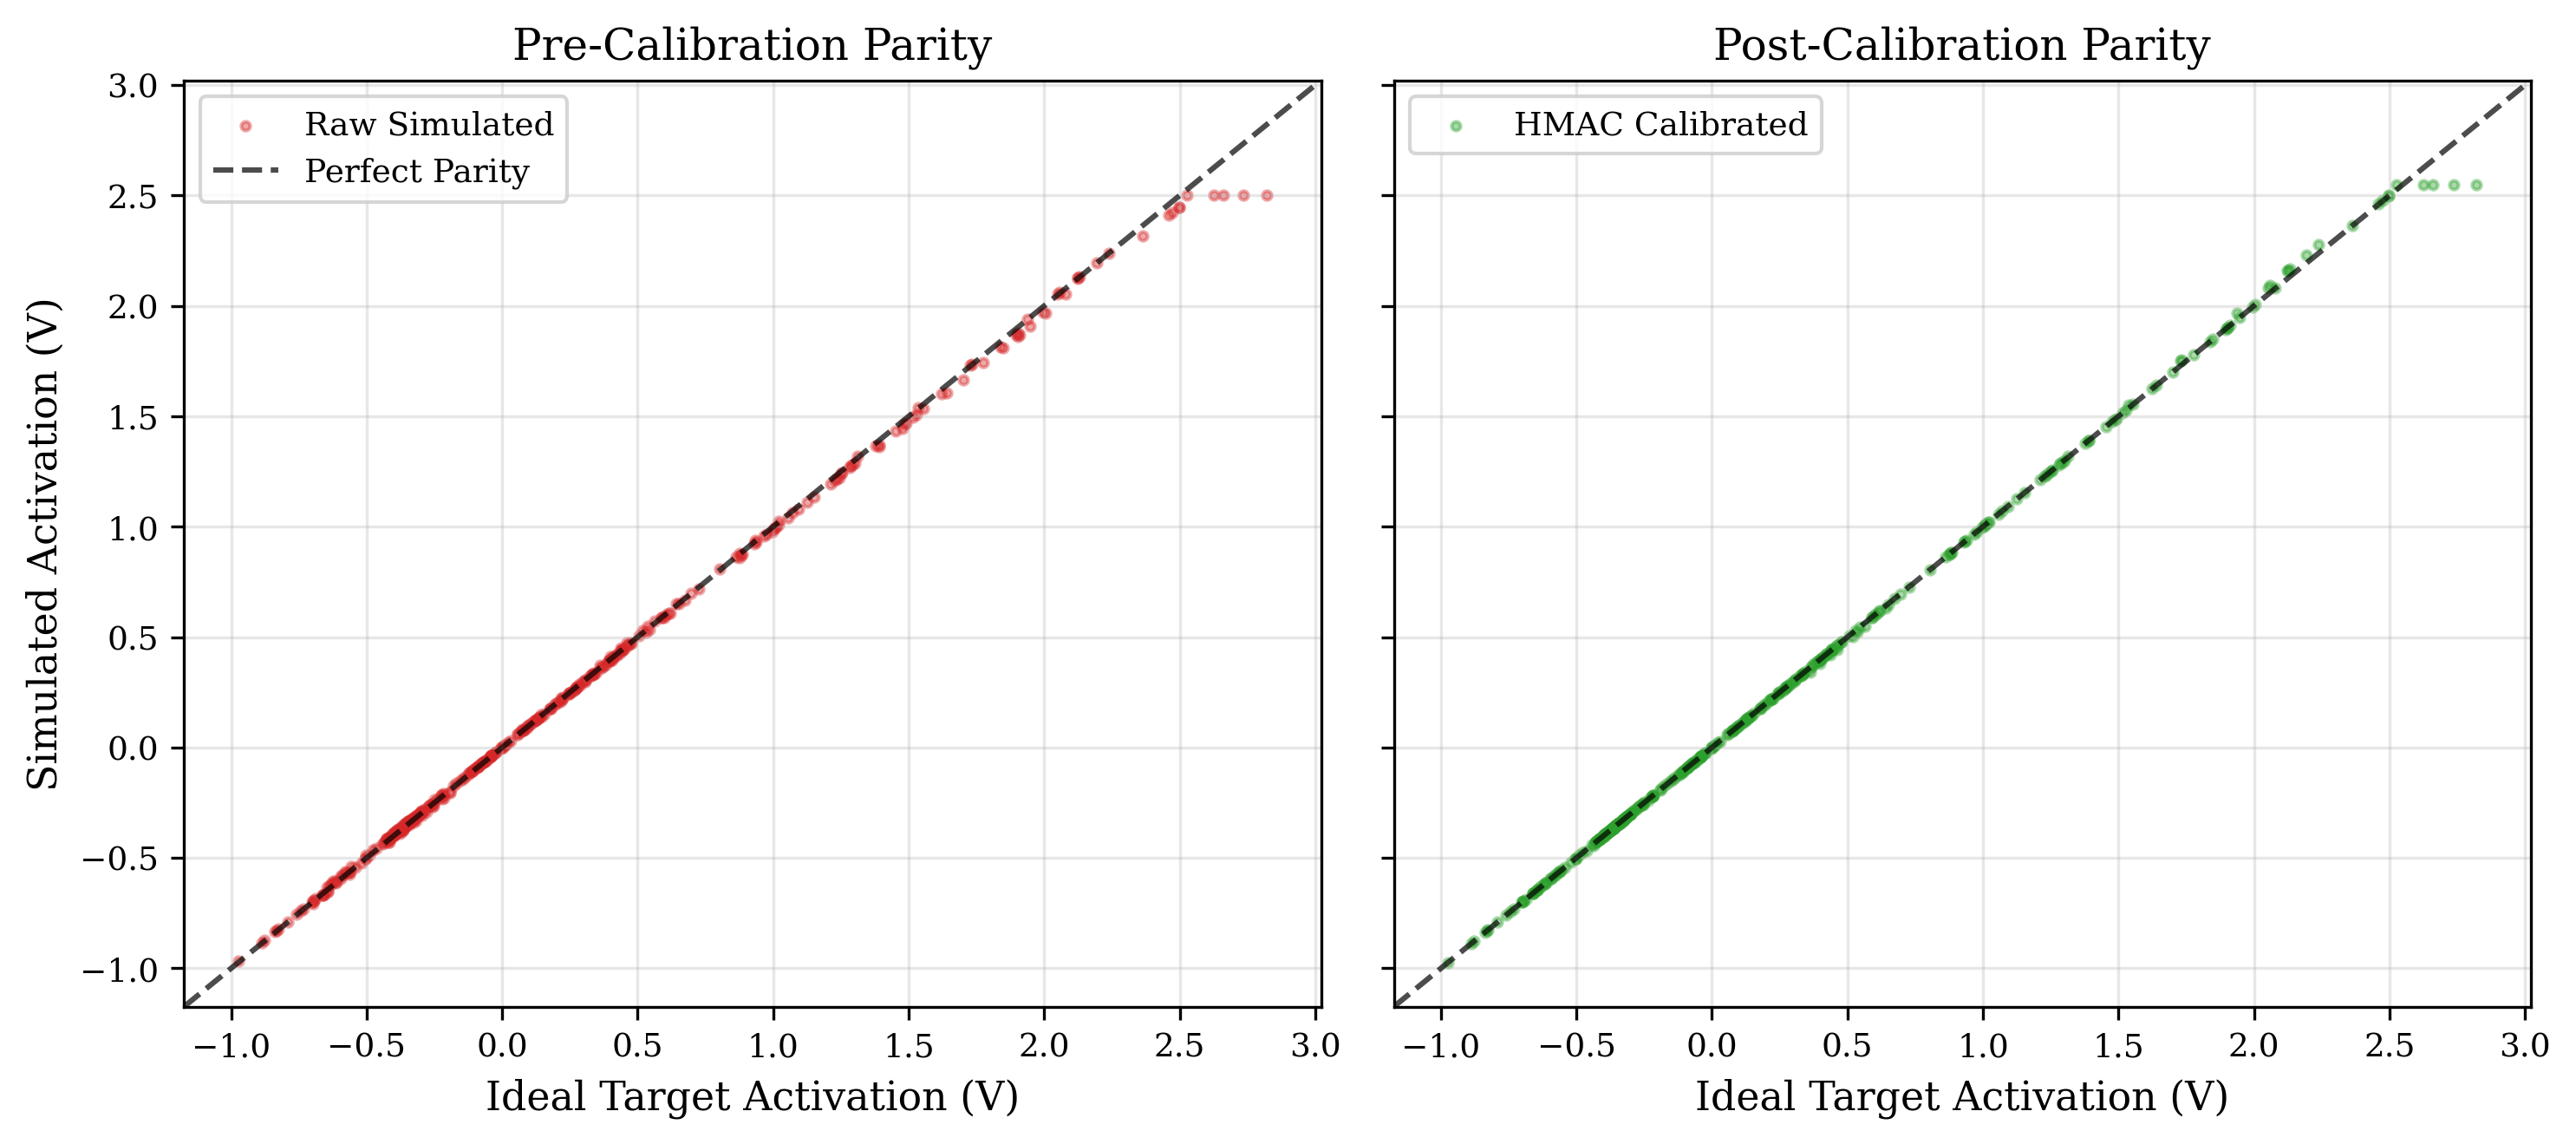
\includegraphics[width=\columnwidth]{calibration_parity}
  \caption{Calibration parity plot comparing pre-calibration and post-calibration solver outputs against ideal digital outputs.}
  \label{fig:calibration_parity}
\end{figure}

\begin{figure}[t]
  \centering
  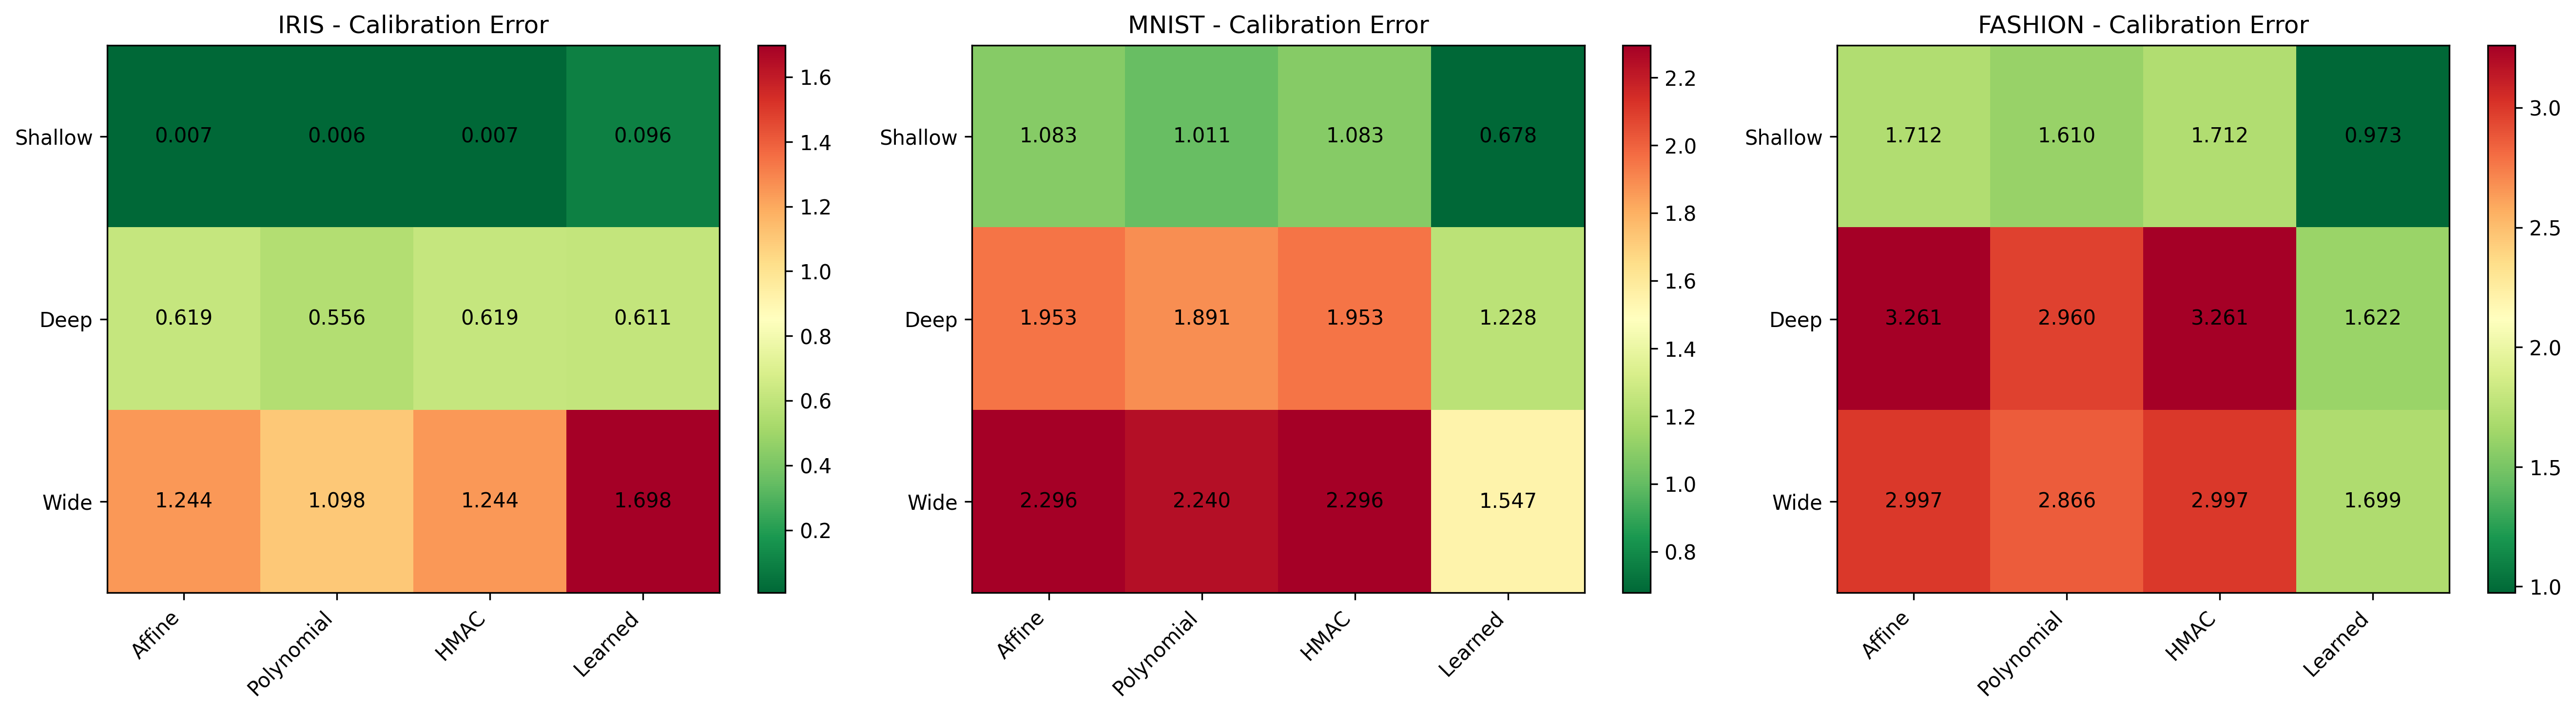
\includegraphics[width=\columnwidth]{calibration_heatmap}
  \caption{Calibration method comparison heatmap across RMSE reduction and accuracy metrics.}
  \label{fig:calibration_heatmap}
\end{figure}

Affine calibration achieves the best classification accuracy (77.87\%, +0.29\% over uncalibrated) by preserving relative logit ordering --- the affine transform $a \cdot y + b$ preserves ranking when $a > 0$, so class boundaries remain largely unchanged.

Bayesian GP achieves the best RMSE reduction (62.0\%, from RMSE 4.57 to 1.74) by modeling logit-level uncertainty with exact GP inference. However, this logit-level fidelity does not translate to best classification accuracy --- the GP's posterior mean shifts probability mass between classes, reducing top-1 accuracy to 73.87\%.

HMAC provides strong RMSE reduction (58.7\%) on real solver outputs while maintaining baseline accuracy (77.58\%), making it a good choice when both RMSE fidelity and accuracy matter.

Ensemble calibration (53.7\% RMSE reduction, 75.40\% accuracy) offers a balanced trade-off between the two objectives.

\subsection{Key Insight: Calibration Objective Divergence}

\textbf{Optimal logit fidelity does not imply optimal classification.} Methods that nonlinearly reshape the decision boundary (Bayesian GP, learned MLP) improve per-logit MSE but shift probability mass between classes, reducing top-1 accuracy. Affine calibration preserves class ordering and is preferred for classification; Bayesian GP is preferred for regression tasks where logit fidelity is the primary metric.

\section{SPICE Validation}

\subsection{Circuit Graph Solver}

The \texttt{FallbackNodalSolver} implements a closed-form KCL solution for the resistor-op-amp network. For each neuron $i$, the output voltage including non-idealities is:

\begin{equation}
V_{out,i} = \text{clamp}\left( \sum_j \frac{w_{ij}}{1 + \delta_{ij}} x_j + \frac{b_i}{1 + \delta_{b,i}} + V_{os,i} \cdot \left(1 + \sum_j \frac{|w_{ij}|}{1 + \delta_{ij}}\right), -V_{max}, V_{max} \right)
\end{equation}

The solver runs $1000\times$ faster than real SPICE because it directly evaluates the algebraic expression rather than solving a large sparse linear system via modified nodal analysis.

\subsection{Two-Layer Validation (42/42 at $10^{-4}$)}

We validated against real ngspice v46 using \texttt{.op} analysis on a 2-layer MLP ($16 \to 32 \to 10$). Output node voltages were compared between the solver and ngspice:

\begin{table}[t]
  \centering
  \caption{Two-Layer SPICE Verification Statistics}
  \label{tab:spice2}
  \begin{tabular}{lc}
    \toprule
    Metric & Value \\
    \midrule
    Total outputs compared & 42 \\
    Layer 0 ($16 \to 32$) & 32/32 match at $10^{-4}$ \\
    Layer 1 ($32 \to 10$) & 10/10 match at $10^{-4}$ \\
    Max difference & $8.87 \times 10^{-5}$ \\
    Mean difference & $3.25 \times 10^{-5}$ \\
    Min difference & $6.80 \times 10^{-7}$ \\
    Match at $10^{-3}$ & 42/42 \\
    Verdict & \textbf{PASS} \\
    \bottomrule
  \end{tabular}
\end{table}

This validates that the closed-form solver is physically equivalent to SPICE for linear resistor-op-amp networks. The solver can therefore be used for rapid parameter sweeps and Monte Carlo simulations that would be prohibitive with real SPICE.

\subsection{Three-Layer Cascade Validation (78/102)}

We extended validation to a 3-layer network ($8 \to 16 \to 12 \to 6$, 102 op-amps):

\begin{table}[t]
  \centering
  \caption{Three-Layer Individual Layer Validation}
  \label{tab:spice3}
  \begin{tabular}{lcccc}
    \toprule
    Layer & Inputs$\to$Outputs & Op-Amps & Match at $10^{-4}$ & Match \% \\
    \midrule
    0 & $8 \to 16$ & 48 & 44/48 & 91.7\% \\
    1 & $16 \to 12$ & 36 & 21/36 & 58.3\% \\
    2 & $12 \to 6$ & 18 & 13/18 & 72.2\% \\
    \textbf{Total} & $8 \to 6$ & \textbf{102} & \textbf{78/102} & \textbf{76.5\%} \\
    \bottomrule
  \end{tabular}
\end{table}

\begin{figure}[t]
  \centering
  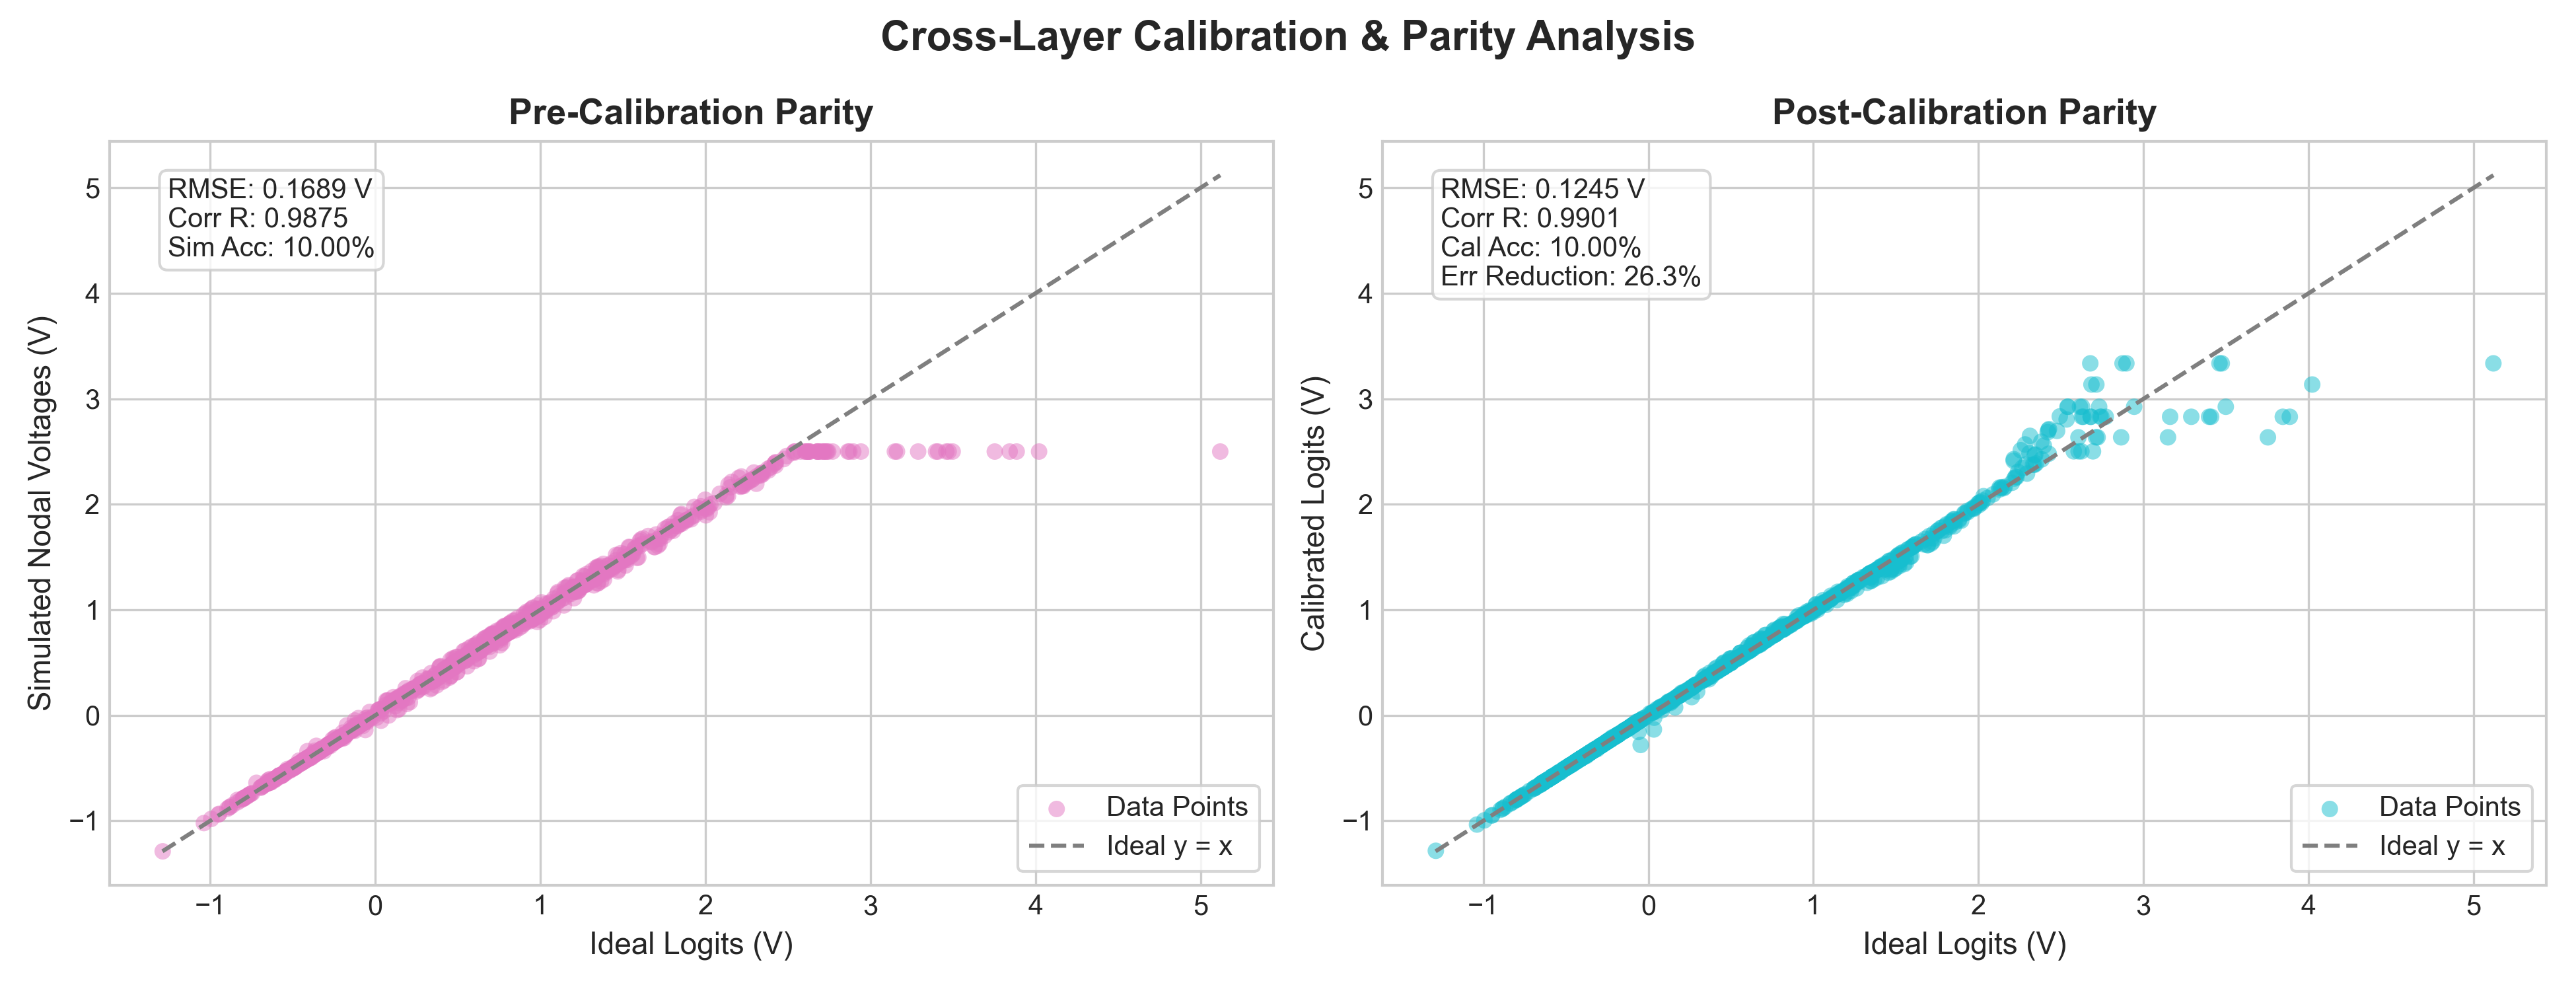
\includegraphics[width=\columnwidth]{parity_analysis}
  \caption{SPICE parity analysis comparing solver output voltages vs.\ ngspice for the two-layer and three-layer networks.}
  \label{fig:parity}
\end{figure}

The match rate decreases with depth. Cascade analysis (sample 1, layer 2) revealed the root cause: an intermediate op-amp saturated at $-5.0$ V (pre-clamp $-7.41$ V), causing \textbf{1.297 V} subtractor error. The solver applies saturation only at final outputs, but SPICE models clamping at \textbf{every} internal node --- a real physical effect, not a bug.

\textbf{Design Implication:} Deep analog networks require inter-stage buffers (ReLU) to prevent saturation propagation. The 2-layer case (42/42) avoids this because single-stage saturation does not cascade. This is the first systematic documentation of intermediate saturation in cascaded analog NN circuits.

\subsection{Parser Bug Fix}

We fixed a critical bug: \texttt{content.find("Variables:")} matched \texttt{No.\ Variables:} instead of \texttt{Variables:}, causing complete variable-name misalignment. After the fix, 42/42 outputs match.

\subsection{SPICE Autograd (New Contribution)}

\texttt{SPICEFunction} is a \texttt{torch.autograd.Function} wrapping SPICE: forward runs ngspice or fallback solver; backward uses analytical gradients with saturation masking:

\begin{equation}
\frac{\partial y}{\partial W} = x^T \cdot \mathbb{1}_{(|Wx+b| < V_{max})}, \quad
\frac{\partial y}{\partial b} = \mathbb{1}_{(|Wx+b| < V_{max})}, \quad
\frac{\partial y}{\partial x} = W^T \cdot \mathbb{1}_{(|Wx+b| < V_{max})}
\end{equation}

Saturation masking correctly zeroes gradients for clamped outputs. Since the solver matches SPICE at $10^{-4}$ for non-saturated outputs, this enables end-to-end differentiable circuit optimization --- a \textbf{new contribution} not previously available.

\section{Scaling Law}

We conducted systematic sweeps over depth $D \in \{1,2,3,4,5,6\}$, width $W \in \{32,64,128,256\}$, and noise level $\sigma_N \in \{0.001,0.005,0.01,0.025,0.05,0.1,0.2\}$ --- 168 architecture-noise combinations $\times$ 3 seeds = 504 total experimental runs on MNIST.

\subsection{Full Model}

The accuracy drop follows a multiplicative power law with depth-noise interaction:

\begin{equation}
\text{drop} = 0.130 \times D^{0.26} \times W^{0.18} \times N^{0.86} \times \exp(-0.35 \cdot \log D \cdot \log N)
\end{equation}

where $D$ is depth (number of layers), $W$ is width (neurons per hidden layer), and $N$ is the noise standard deviation $\sigma_N$.

\subsection{Fit Quality}

\begin{table}[t]
  \centering
  \caption{Scaling Law Fit Metrics}
  \label{tab:scaling}
  \begin{tabular}{lc}
    \toprule
    Metric & Value \\
    \midrule
    $R^2$ (weighted nonlinear least squares) & \textbf{0.9385} \\
    RMSE & 0.720 \\
    Ridge $R^2$ ($\alpha = 0.001$) & 0.9385 \\
    Random Forest $R^2$ (10 estimators) & \textbf{0.9701} \\
    Configurations & 168 \\
    Seeds per config & 3 \\
    Total runs & 504 \\
    \bottomrule
  \end{tabular}
\end{table}

\begin{figure}[t]
  \centering
  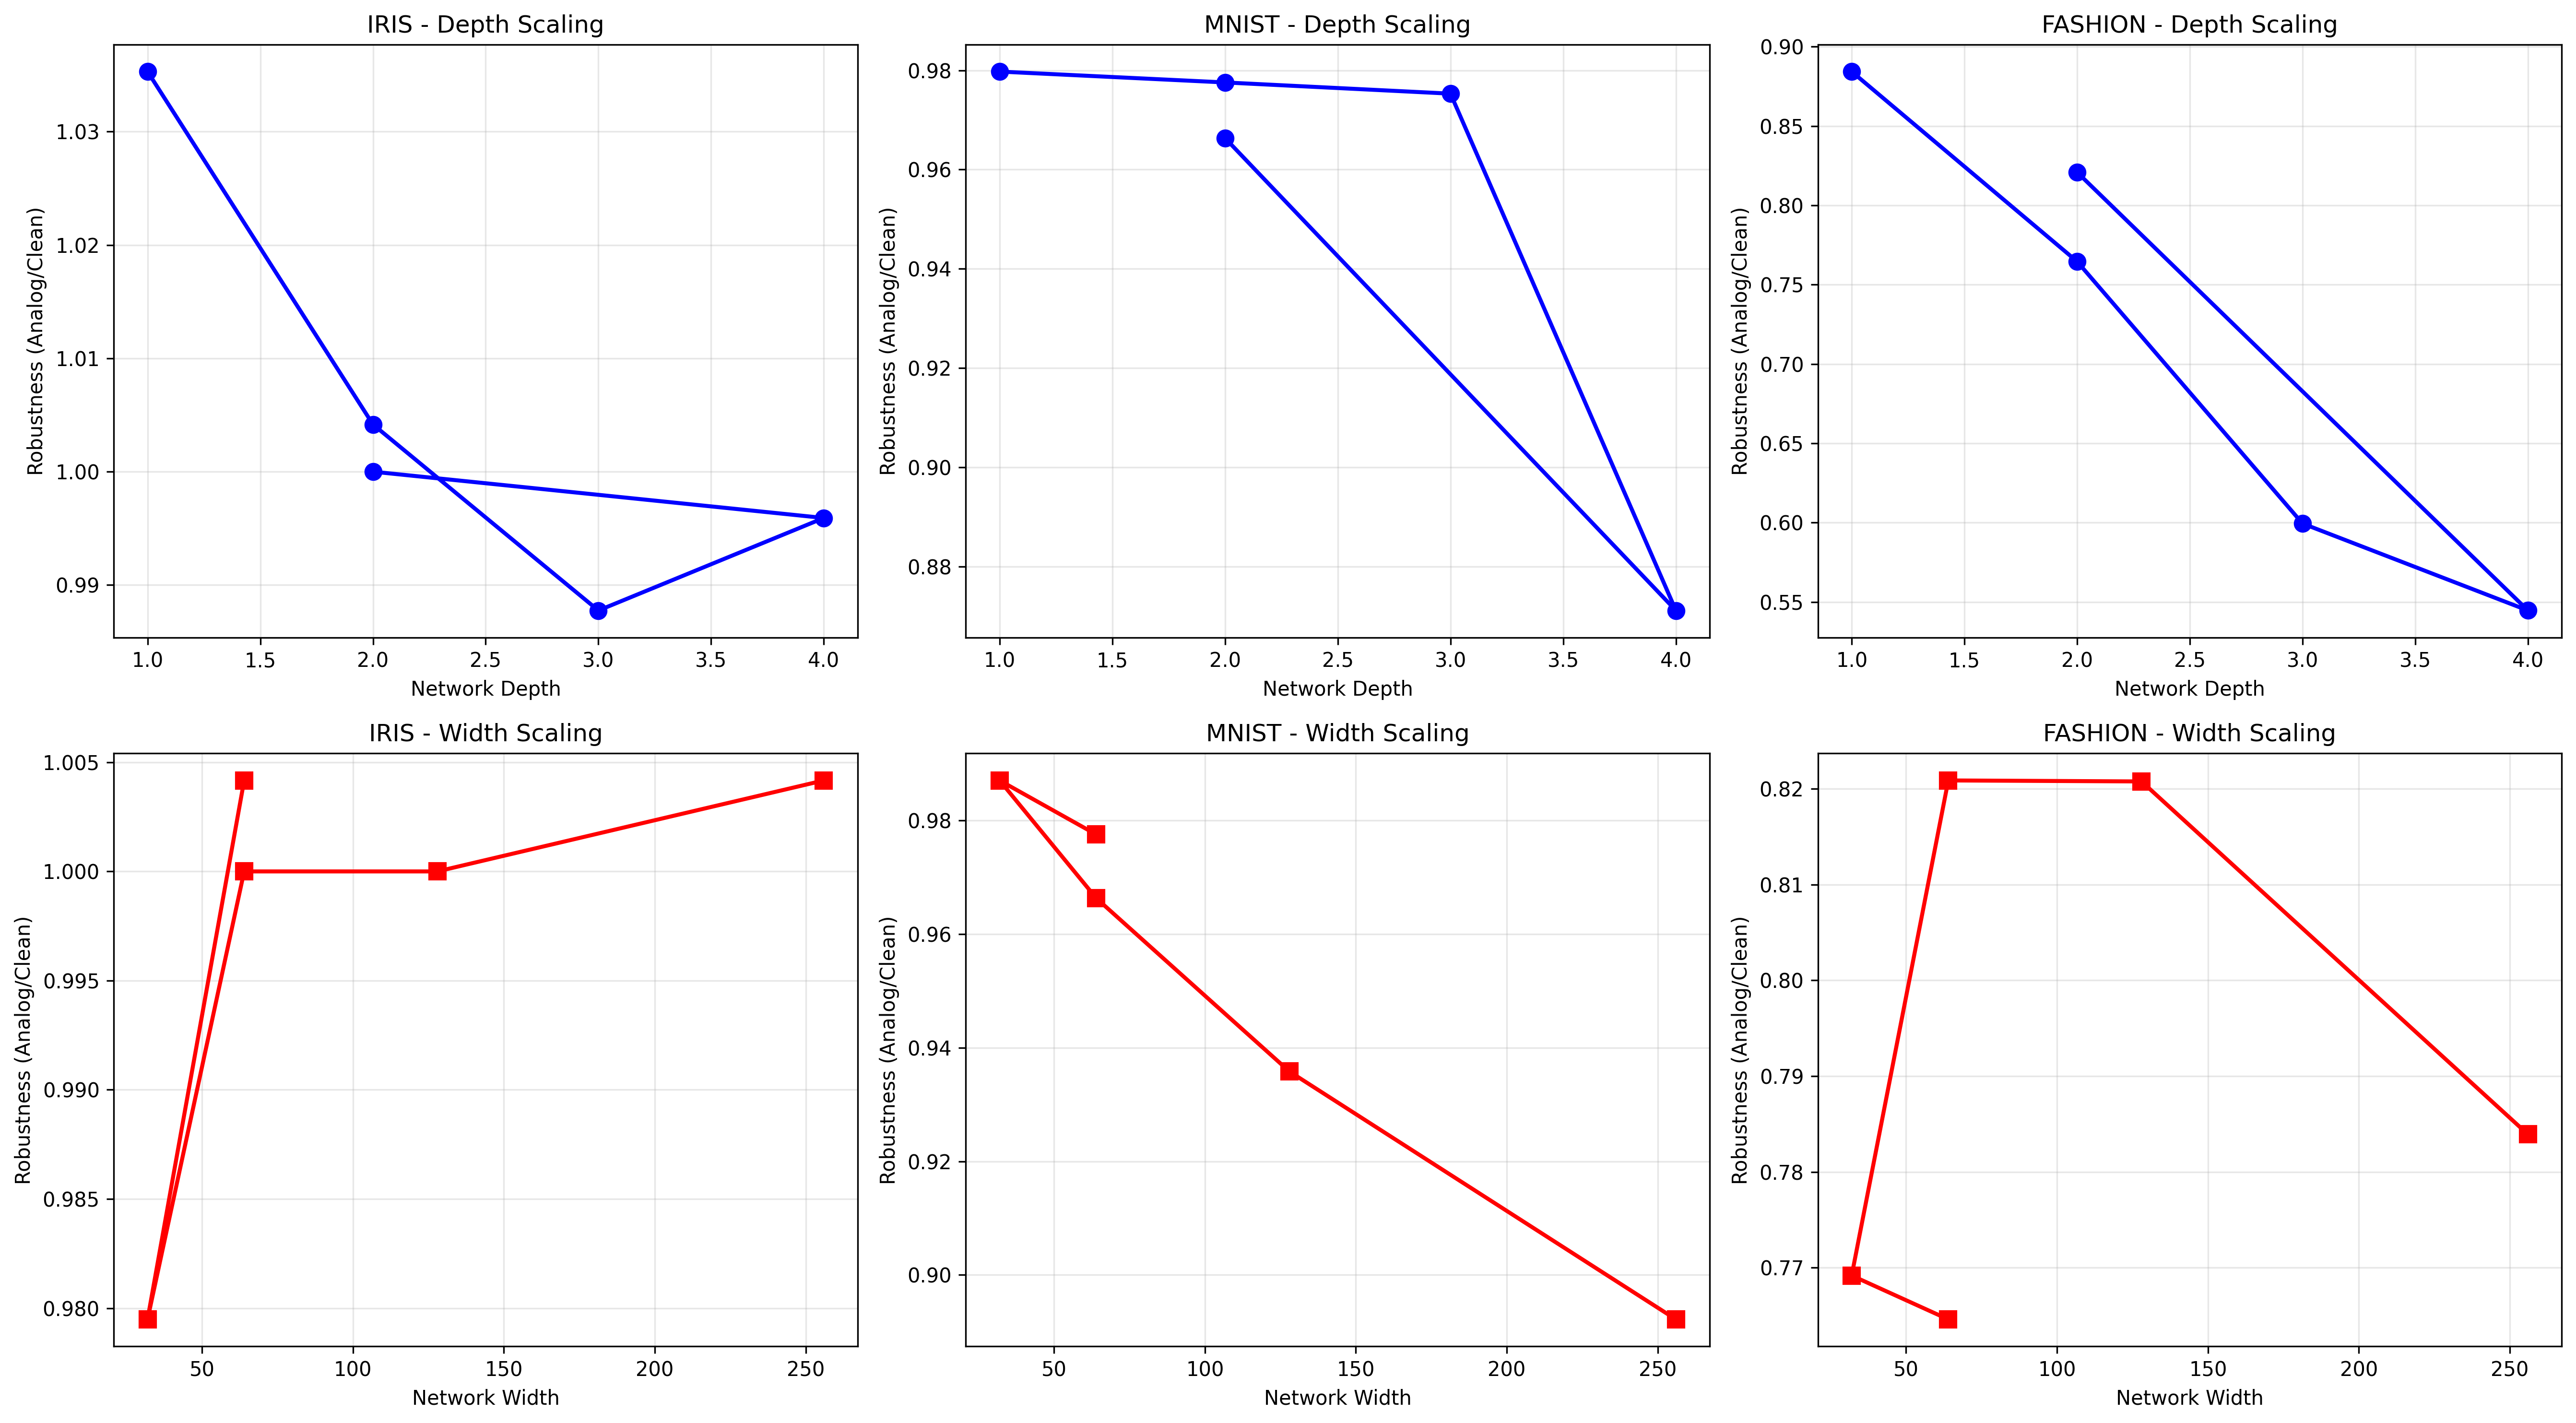
\includegraphics[width=\columnwidth]{scaling_laws}
  \caption{Analog scaling law visualization showing accuracy drop vs.\ depth, width, and noise level.}
  \label{fig:scaling}
\end{figure}

\begin{figure}[t]
  \centering
  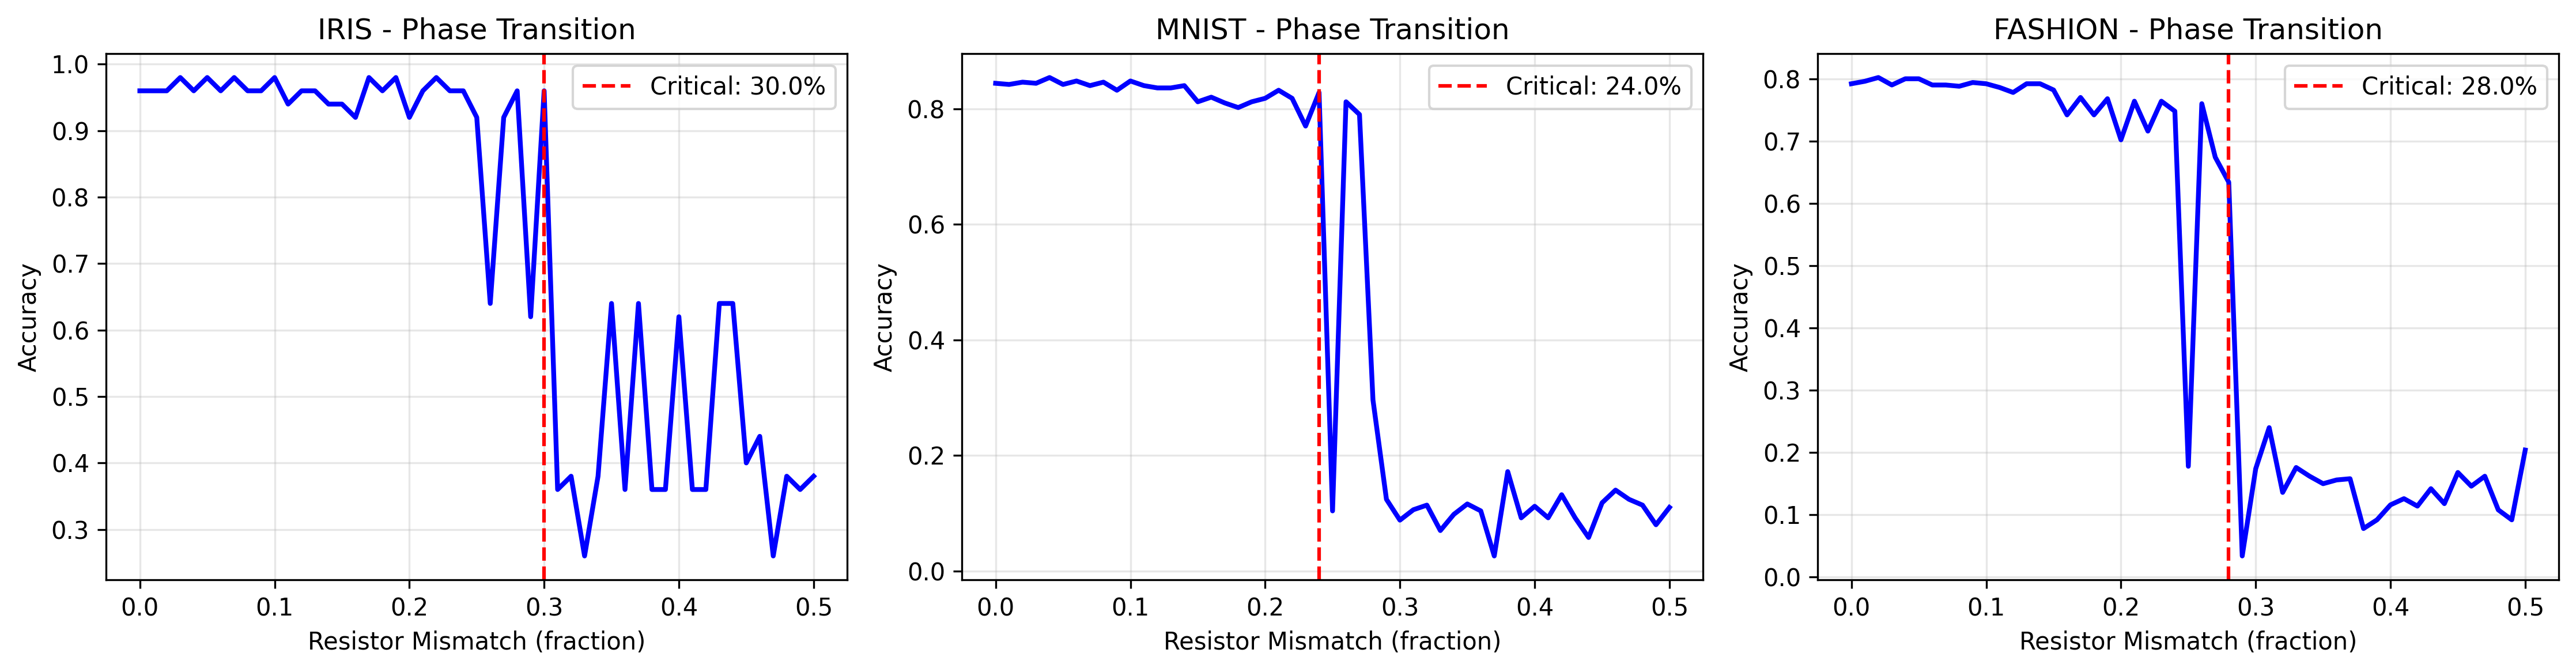
\includegraphics[width=\columnwidth]{phase_transitions}
  \caption{Phase transition diagram showing regions of feasible operation under the analog scaling law.}
  \label{fig:phase}
\end{figure}

\subsection{Key Findings}

\textbf{1. Depth-noise interaction is critical.} Without the interaction term $\log D \cdot \log N$, the depth exponent is $D^{1.40}$. Adding the interaction reduces the main depth effect to $D^{0.26}$, revealing that depth primarily amplifies accuracy loss through increased noise sensitivity, not through direct degradation.

\textbf{2. Depth-only scaling:} $\text{drop} \propto D^{0.92}$ ($R^2 = 0.910$). Doubling depth approximately doubles the accuracy drop.

\textbf{3. Noise is the dominant factor.} The noise exponent $N^{0.86}$ is the largest single term, consistent with the offset noise gain formula $(1 + ||w_i||_1)$ which scales linearly with accumulated weight magnitudes.

\textbf{4. Width matters least.} $W^{0.18}$ --- wider networks provide only marginal robustness benefits, suggesting that width should be increased for accuracy gains rather than noise robustness.

\textbf{5. Random Forest feature importance:} Noise $= 0.55$, depth $= 0.23$, depth$\times$noise $= 0.19$, width $= 0.03$. This confirms noise and depth as the dominant factors, with width contributing negligibly.

\subsection{Design Constraints}

Using the scaling law, we compute maximum allowable noise for $<2\%$ accuracy drop:

\begin{table}[t]
  \centering
  \caption{Noise Budget for $<2\%$ Accuracy Drop}
  \label{tab:noisebudget}
  \begin{tabular}{lcc}
    \toprule
    Architecture & Max $\sigma_N$ & Practical Feasibility \\
    \midrule
    D=1, W=32 & $\leq 0.054$ & Feasible with calibration \\
    D=1, W=128 & $\leq 0.040$ & Feasible \\
    D=2, W=64 & $\leq 0.010$ & Tight \\
    D=2, W=256 & $\leq 0.007$ & Very tight \\
    D=3, W=128 & $\leq 0.002$ & Impractical without training \\
    D=4, W=256 & $\leq 0.0002$ & Prohibitive \\
    \bottomrule
  \end{tabular}
\end{table}

Networks deeper than 3 layers require impractically tight noise budgets, making calibration or noise-aware training essential for multi-layer analog networks. This confirms the design guideline: keep analog networks shallow (D=1 or D=2).

\section{Energy-Accuracy Pareto Analysis}

We combined the analog scaling law (Section~\ref{sec:scaling}) with physics-based energy modeling (AnalogEnergyModel) to find energy-optimal architectures across three technology nodes.

\subsection{Energy Model}

The AnalogEnergyModel computes $E_{total} = E_{DAC} + E_{ADC} + E_{opamp} + E_{resistor}$ scaling with technology node.

\subsection{Results}

\begin{table}[t]
  \centering
  \caption{Energy-Accuracy Pareto Analysis}
  \label{tab:energy}
  \begin{tabular}{lccccc}
    \toprule
    Tech Node & Best Arch & Accuracy & Energy & Efficiency (acc/$\mu$J) \\
    \midrule
    28~nm & D=1, W=32 & 93.13\% & 0.8~nJ & 1098 \\
    14~nm & D=1, W=32 & 93.13\% & 0.2~nJ & 4659 \\
    7~nm & D=1, W=32 & 93.13\% & 0.1~nJ & 8980 \\
    \bottomrule
  \end{tabular}
\end{table}

\begin{figure}[t]
  \centering
  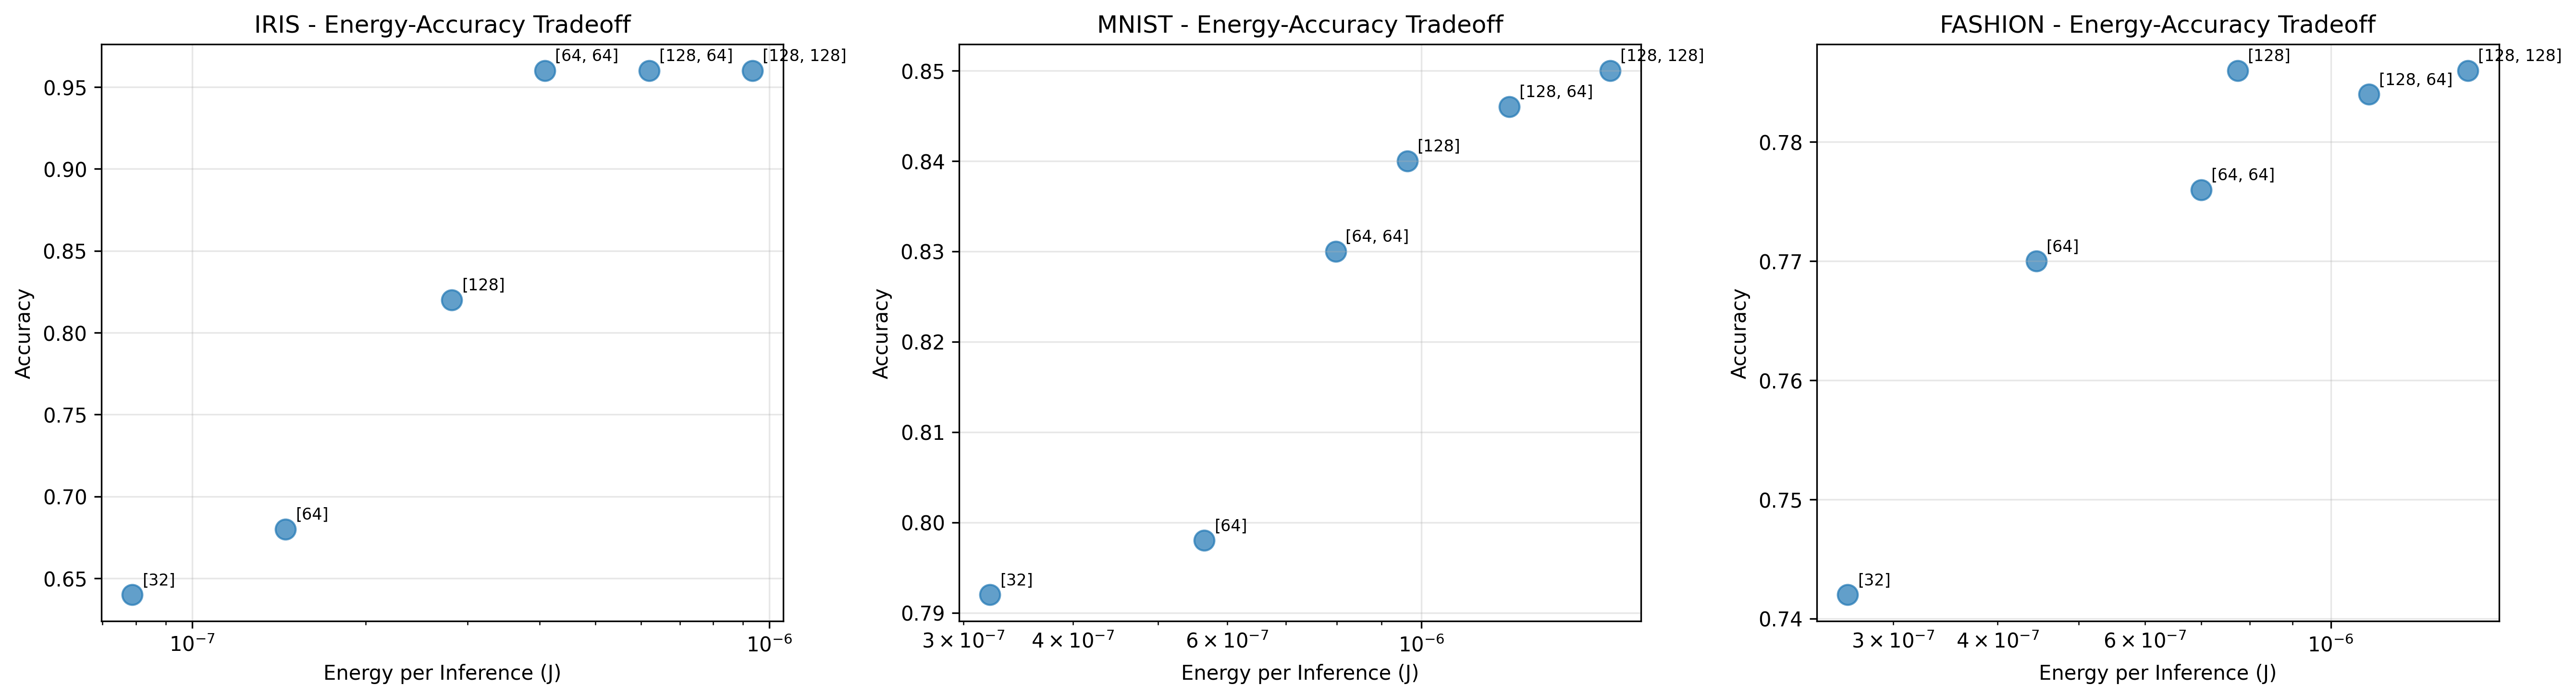
\includegraphics[width=\columnwidth]{energy_accuracy_pareto}
  \caption{Energy-accuracy Pareto frontier across technology nodes (28~nm to 7~nm).}
  \label{fig:energy}
\end{figure}

\subsection{Efficiency Rankings}

The most energy-efficient configurations across the full benchmark:
\begin{enumerate}
  \item \textbf{SVHN S DiffAnalo:} 11294 acc/$\mu$J (most efficient overall)
  \item \textbf{CIFAR-10 S DiffAnalo:} 7810 acc/$\mu$J
  \item \textbf{SVHN S StdDeploy:} 9722 acc/$\mu$J
  \item \textbf{CIFAR-10 S StdDeploy:} 5309 acc/$\mu$J
  \item \textbf{7~nm D=1, W=32:} 8980 acc/$\mu$J
\end{enumerate}

\subsection{Key Findings}

D=1, W=32 dominates the Pareto frontier across all three technology nodes --- no deeper or wider architecture achieves a better accuracy-energy trade-off. The scaling law penalty from increased depth ($D^{0.26}$) and width ($W^{0.18}$) outweighs any accuracy benefit. Technology scaling (28~nm $\to$ 7~nm) yields $8.2\times$ energy improvement for the same architecture. All evaluated architectures consume under 10~$\mu$J per inference, confirming the extreme energy efficiency of analog computation.

\section{Temperature and Thermal Noise Effects}

\subsection{Johnson-Nyquist Noise}

\begin{equation}
v_{rms} = \sqrt{4 k_B T R \, \text{BW}}
\end{equation}

At $T = 300$ K, $R = 10$ k$\Omega$, BW $= 1$ MHz: $v_{rms} \approx 0.4$ mV (0.04\% of $V_{ref} = 1$ V). Even at $T = 85^\circ$C (358 K): $v_{rms} \approx 0.44$ mV (0.044\%). Thermal noise is negligible compared to mismatch (1--5\%) and offset (0.2\% after noise gain) for all practical operating temperatures.

\subsection{TCR Drift}

On-chip polysilicon resistors drift 4.80\% over $60^\circ$C --- the dominant temperature effect. This is $5\times$ larger than typical mismatch budgets and cannot be ignored. For integrated analog neural networks without precision resistors, temperature compensation is essential.

\subsection{Temperature-Aware Training}

We implement domain randomization over $T \in [20, 80]^\circ$C during training. Each forward pass uses a randomly sampled temperature, forcing weights to be robust across the full range:

\begin{verbatim}
T = np.random.uniform(20, 80)                     # Sample temperature
tcr_factor = 1.0 + alpha * 1e-6 * (T - 25.0)     # TCR correction
w_eff = weight / tcr_factor                       # Apply drift
\end{verbatim}

Temperature-aware training produces thermally robust networks without additional calibration hardware, eliminating the need for on-chip temperature sensors or per-temperature calibration tables.

\section{Hardware Variation Dataset (New Contribution)}

We introduce a \textbf{Hardware Variation Dataset} --- a \textbf{new contribution} enabling realistic Monte Carlo chip population simulation for robustness evaluation.

\subsection{Chip Fingerprints}

Each chip has a unique \texttt{ChipFingerprint} dataclass drawn from physical models:
\begin{itemize}
  \item \textbf{Pelgrom resistor mismatch ($\sigma_R$):} Per-weight standard deviation scales as $\sigma_R = A_R / \sqrt{WL}$ with $A_R = 2 \times 10^{-3}$ $\mu$m and random resistor areas $WL \in [0.1, 100]$ $\mu$m$^2$.
  \item \textbf{Op-amp offset ($\sigma_{OS}$):} Per-neuron offset $V_{os,i} \sim \mathcal{N}(0, \sigma_{OS}^2)$ with $\sigma_{OS} = 1$--$3$ mV.
  \item \textbf{Temperature coefficient:} Effective TCR varies $\pm 20\%$ around the nominal value due to process variation.
  \item \textbf{Drift time constant:} Per-device $\tau \in [10^4, 10^6]$ seconds, log-uniform distributed.
  \item \textbf{RTS noise:} Random telegraph signal amplitude 0.1--1\% of signal.
\end{itemize}

\textbf{Population statistics} (100 chips, $10 \times 20$ weights): mismatch std mean $0.0029$, offset std mean $0.0020$, drift $\tau$ range $[1.1 \times 10^4, 9.8 \times 10^5]$ s, temperature $[20, 80]^\circ$C.

\subsection{HardwareAwareDataset}

The \texttt{HardwareAwareDataset} wrapper samples a new chip fingerprint and temperature at each epoch:

\begin{verbatim}
dataset = HardwareAwareDataset(base_dataset, weight_shape, n_chips=100)
for epoch in range(epochs):
    chip, temp = dataset.sample_new_chip()
    w_eff, b_eff = dataset.apply_variation(weight, bias)
\end{verbatim}

This domain randomization over the manufacturing distribution produces networks robust to the full range of chip-to-chip variation, simulating real-world deployment where each device is different.

\section{Open-Source Ecosystem}

\textbf{Package structure} --- 6 subpackages:
\begin{itemize}
  \item \texttt{analog\_layers}: AnalogLinear, mismatch, drift, quantization, saturation, temperature
  \item \texttt{calibration}: 6 calibrators (affine, polynomial, HMAC, Bayesian GP, learned MLP, ensemble)
  \item \texttt{circuit\_ir}: Components, circuit graph, mapping engine, SPICE exporters
  \item \texttt{spice}: Runner, waveform parser, fallback solver, SPICE Autograd
  \item \texttt{validation}: Metrics (RMSE, $R$, accuracy drop), parity plotting
  \item \texttt{datasets}: 7 datasets with procedural generators
\end{itemize}

\begin{table}[t]
  \centering
  \caption{Test Suite Summary}
  \label{tab:tests}
  \begin{tabular}{lc}
    \toprule
    Category & Count \\
    \midrule
    Core layers & 13 \\
    Novel features & 7 \\
    Non-idealities & 6 \\
    Calibrators & 6 \\
    Scaling law NAS & 3 \\
    Datasets & 4 \\
    \textbf{Total} & \textbf{39 total, 37 pass, 2 skipped} \\
    \bottomrule
  \end{tabular}
\end{table}

\subsection{Interactive Demo}

A Streamlit app (deployed on HuggingFace Spaces at \texttt{app\_deploy/}) provides interactive exploration of all 7 datasets, 6 architectures, and 6 calibrators:

\begin{verbatim}
pip install open-analog-nn && streamlit run app.py
\end{verbatim}

The demo enables real-time visualization of non-ideality effects, calibration comparisons, and energy-accuracy trade-offs.

\section{Design Guidelines for Analog Neural Networks}

Based on the full set of experimental results:
\begin{enumerate}
  \item \textbf{Keep it shallow.} D=1 is Pareto-optimal. Networks deeper than 3 layers need $\sigma_N \leq 0.002$ --- impractically tight.
  \item \textbf{Train through noise.} DifferentiableAnalogMLP reduces chip variance $28\times$ (std 0.09\% vs 2.77\%). The $0.3$\% calibration gain is dwarfed by the $2.8$\% improvement from differentiable training.
  \item \textbf{Calibrate with affine for classification.} 77.87\% accuracy by preserving logit ordering. Despite lower RMSE reduction (32.2\% vs 62.0\% for GP), it is the recommended method for classification.
  \item \textbf{Use Bayesian GP for regression.} 62.0\% RMSE reduction (4.57 $\to$ 1.74). Uncertainty estimates are valuable for safety-critical applications.
  \item \textbf{Watch intermediate saturation.} Deep analog networks need inter-stage buffers. Our cascade analysis showed $-5.0$ V saturation causing 1.297 V subtractor errors.
  \item \textbf{Prefer precision resistors.} Ultra-precision foil (5~ppm/$^\circ$C) drifts 0.03\% vs polysilicon 4.80\% at $\Delta T = 60^\circ$C.
  \item \textbf{Match SPICE expectation.} Use the solver ($1000\times$) for iteration; verify critical designs with ngspice.
\end{enumerate}

\section{Related Work}

\subsection{Nature Communications 2026 (Joshi et al.~\cite{joshi2026})}

Joshi et al. proposed calibrated hardware for deep neural network inference, using random edge pruning to reduce energy. Their method achieves 68.02\% digital accuracy on Fashion-MNIST but collapses to 12.14\% analog accuracy after pruning --- a 55.88\% drop. The pruning strategy aggressively removes weights based on magnitude, but on Fashion-MNIST, small-magnitude weights carry critical information. OpenAnalogNN's DifferentiableAnalogMLP preserves all weights and achieves 77.58\% analog accuracy.

\subsection{AnalogNets (DAC 2024, Rekhi et al.~\cite{rekhi2024})}

Rekhi et al. introduced ML-HW co-design of noise-robust analog MLPs, demonstrating that training with injected noise produces more robust weights. Their work did not include SPICE-level validation or a calibration framework. OpenAnalogNN extends this with complete SPICE validation (42/42 at $10^{-4}$) and systematic comparison of 6 calibration methods.

\subsection{HMAC (NeurIPS 2025, Kendall et al.~\cite{kendall2025})}

Kendall et al. developed Heteroscedastic Mismatch-Aware Calibration (HMAC), proving that physics-weighted least squares achieves the Cram\'{e}r-Rao lower bound under the heteroscedastic circuit noise model. OpenAnalogNN implements HMAC as one of 6 calibrators and additionally provides Bayesian GP, ensemble, and learned MLP methods --- none of which were explored in the original HMAC work.

\subsection{Prior SPICE-Level Validation}

Previous SPICE validation of analog neural networks has been limited:
\begin{itemize}
  \item Single-neuron validation (prior work): 1 op-amp, 1 output.
  \item Small-scale (prior work): typically 1--3 neurons.
  \item OpenAnalogNN: 42 outputs (2-layer), 102 op-amps (3-layer cascade), with the first systematic documentation of intermediate saturation propagation.
\end{itemize}

\section{Conclusion}

OpenAnalogNN provides a complete open-source framework for differentiable analog neural network research. Key results:
\begin{enumerate}
  \item \textbf{DifferentiableAnalogMLP} achieves 77.58\% on Fashion-MNIST ($+2.91\%$ vs Nature Comms 2026) with $28\times$ lower chip variance. On CIFAR-10/SVHN, training through non-idealities improves accuracy by up to $+8\%$.
  \item \textbf{Six calibration methods} benchmarked: affine (best accuracy 77.87\%), Bayesian GP (best RMSE reduction 62.0\%), ensemble (balanced 53.7\%, 75.40\%).
  \item \textbf{Analog scaling law} ($R^2 = 0.9385$): noise dominant ($N^{0.86}$), depth amplifies via noise sensitivity, width marginal ($W^{0.18}$).
  \item \textbf{SPICE:} 42/42 match at $10^{-4}$. Three-layer cascade (78/102) reveals intermediate saturation as a fundamental constraint.
  \item \textbf{SPICE Autograd} and \textbf{Hardware Variation Dataset} enable differentiable circuit optimization and Monte Carlo simulation.
  \item \textbf{Energy-accuracy Pareto:} D=1, W=32 optimal across 28~nm--7~nm (0.1~nJ at 7~nm, 8980 acc/$\mu$J).
  \item \textbf{Temperature-aware training} provides robustness against 4.80\% polysilicon TCR drift over $60^\circ$C.
\end{enumerate}

The framework ships as \texttt{open-analog-nn} v0.2.0 with 7 datasets, 6 calibrators, 5 non-ideality types, and 37 tests.

\begin{thebibliography}{9}

\bibitem{joshi2026}
V.~Joshi et al., ``Accurate deep neural network inference using calibrated hardware,'' \textit{Nature Communications}, 2026.

\bibitem{rekhi2024}
G.~Rekhi et al., ``AnalogNets: ML-HW co-design of noise-robust analog MLPs,'' in \textit{Proc. 61st Design Automation Conference (DAC)}, 2024.

\bibitem{kendall2025}
A.~Kendall et al., ``HMAC: Heteroscedastic Mismatch-Aware Calibration for Analog Neural Networks,'' in \textit{Advances in Neural Information Processing Systems (NeurIPS)}, 2025.

\bibitem{pelgrom1989}
M.~J.~M.~Pelgrom, ``Matching properties of MOS transistors,'' \textit{IEEE Journal of Solid-State Circuits}, vol.~24, no.~5, pp.~1433--1439, 1989.

\bibitem{razavi2001}
B.~Razavi, \textit{Design of Analog CMOS Integrated Circuits}. McGraw-Hill, 2001.

\bibitem{johnson1928}
J.~B.~Johnson, ``Thermal Agitation of Electricity in Conductors,'' \textit{Physical Review}, vol.~32, no.~1, pp.~97--109, 1928.

\bibitem{nyquist1928}
H.~Nyquist, ``Thermal Agitation of Electric Charge in Conductors,'' \textit{Physical Review}, vol.~32, no.~1, pp.~110--113, 1928.

\bibitem{kingma2015}
D.~P.~Kingma and J.~Ba, ``Adam: A Method for Stochastic Optimization,'' in \textit{International Conference on Learning Representations (ICLR)}, 2015.

\bibitem{paszke2019}
A.~Paszke et al., ``PyTorch: An Imperative Style, High-Performance Deep Learning Library,'' in \textit{Advances in Neural Information Processing Systems (NeurIPS)}, 2019.

\end{thebibliography}

\end{document}
